\documentclass[urop]{socreport}
\usepackage{fullpage}
\usepackage{amsmath}
\usepackage{amssymb}
\usepackage{graphicx}
\usepackage{hyperref}
\usepackage[ruled,vlined]{algorithm2e}
\begin{document}
\pagenumbering{roman}
\title{Algorithms for Online Task Assignment Problem}
\author{Tan Wei Yang}
\projyear{2019/20}
\projnumber{U038730}
\advisor{Dr. Leong Hon Wai}
\deliverables{
	\item Report: 1 Volume
	\item Source Code: 1 .zip file}

\newcommand{\A}{\mathcal{A}}
\newcommand{\R}{\mathcal{R}}
\newcommand{\W}{\mathcal{W}}
	
\maketitle
\begin{abstract}
In this report, we study a variant of online task assignment, the minimum fleet problem. We study the effect of four algorithms, the Greedy, Random, Ranking and Highest Redundancy algorithms on the minimum fleet size under the constraint of fulfilling a 99\% of requests under a maximum delay. The study is done in various settings under a Cartesian plane using real-world and synthetic data. We find that the minimum fleet size is the largest for the Greedy algorithm under the settings studied where the spatial distribution of requests is not uniform. The Ranking algorithm leads to a higher minimum fleet size compared to the Random algorithm in most of the settings studied. The Highest Redundancy algorithm shows promise, but does not perform as well as the Random and Ranking algorithms when the spatial distribution is not uniform. Following these results, we discuss the contributing factors to the observations, as well as changes that can be made to the Highest Redundancy algorithm.

\begin{descriptors}
    \item Online Algorithms
    \item Experimentation
\end{descriptors}
\begin{keywords}
	Online Task Assignment, Minimum Fleet Problem
\end{keywords}
\begin{implement}
	CentOS 7.x, Python 3.7
\end{implement}
\end{abstract}

\begin{acknowledgement}
   I would like to thank my supervisor, Professor Leong Hon Wai, as well as Melvin Zhang for the guidance given in this project. I would also like to express gratitude for my friends and family, without whom I would not have been able to complete this project.
\end{acknowledgement}

\listoffigures 
\listoftables
\tableofcontents 

\chapter{Introduction}
In this chapter, we first give the motivation for the online task assignment and the variant we are studying, the minimum fleet problem. Following that, we give the background for the minimum fleet problem and an associated problem, spatial crowdsourcing. We conclude this chapter with an overview of how this report is organized.

\section{Motivation}
Online task assignment(OTA) is a ubiquitous problem. From courier services to transport systems that utilize crowdsourcing like Grab, we require algorithms to assign service providers to users. We ultimately focus on the context of a firm that hires a fleet of service providers to satisfy requests from users, similar to a taxi or a delivery company. In this context, the service provided consists of moving a person or object from a start location to an end location. A major source of operational costs for firms providing such services is the cost of hiring a fleet of workers to meet service requests. Hence, we ultimately seek to minimize the size of the fleet, while keeping to certain constraints. 

The constraint we have decided to look at is a maximum delay between the time of creation of a service request and the time at which a worker starts to fulfil the request. This is akin to providing a guarantee on the maximum waiting time, much like delivery time guarantees for real world products. To account for outliers in the set of requests to be fulfilled, we soften the maximum delay constraint to allow a small number (1\%) of requests to exceed the maximum delay.

\section{Background}
In this section, we briefly discuss the history and background
of the problem. A detailed literature survey is presented in 
Chapter \ref{ch:related}.

\subsection{Illustration of Online Task Assignment}
We can view OTA as a problem of assigning taxi drivers (workers) to customers (requests) who call-in for taxi services.

\begin{figure}
    \centering
    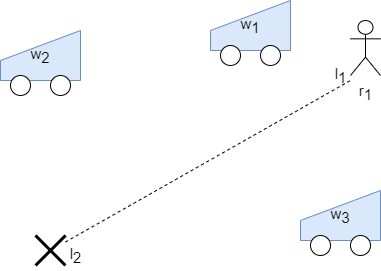
\includegraphics[scale=0.6]{FYP-LaTeX-Template/images/ota_basic.png}
    \caption{Example of OTA}
    \label{fig:idle}
\end{figure}

In this scenario, we will receive a stream of taxi service requests from customers. Every time a request is received, we assign a taxi driver to it immediately. Figure \ref{fig:idle} shows the time slice when the request $r$ to move from location $l_1$ to $l_2$ is received. We can assign any of the taxi drivers $w_i$ to fulfill this request.

\begin{figure}
    \centering
    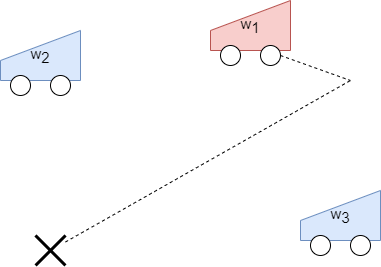
\includegraphics[scale=0.6]{FYP-LaTeX-Template/images/ota_assign.png}
    \caption{Assigning a worker}
    \label{fig:assign}
\end{figure}

Suppose $w_1$ is assigned to $r_1$. Then $w_1$ will be move towards $l_1$ to pick up the customer, and move to $l_2$ to drop off the customer at the destination, as shown in Figure \ref{fig:assign}. In our problem, we assume that taxi drivers only move to fulfill requests, and are otherwise stationary.


In our problem, it is also possible to assign a taxi driver who is still assigned to some other customer to a new customer. As depicted in Figure \ref{fig:nonidle}, even though $w_1$ is still busy, it is arguably reasonable to assign $w_1$ to $r_2$ as $w_1$ is about to complete its current assignment and would be the closest to $r_2$.

\begin{figure}
    \centering
    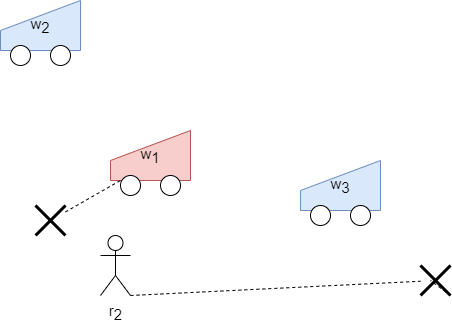
\includegraphics[scale=0.6]{FYP-LaTeX-Template/images/ota_nonidle.png}
    \caption{Example of OTA with Non-idle Workers}
    \label{fig:nonidle}
\end{figure}

\subsubsection{Maximum Delay and Minimum Fleet Problem}
Of course, as customers we want to reach our destination as fast as possible. While we can study the time at which the taxi driver drops off the customer, it is also equivalent to study the time at which the taxi driver picks up the customer. This is because the travel time would be the same in this problem, as the same path (a straight line from source to destination) is used. This also assumes that all taxi drivers have the same velocity when moving.

\begin{figure}[h]
    \centering
    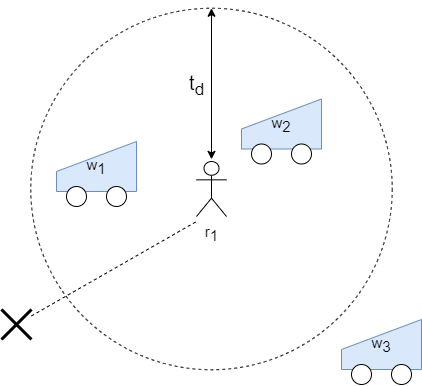
\includegraphics[scale=0.6]{FYP-LaTeX-Template/images/ota_delay.png}
    \caption{A Representation of Maximum delay in OTA}
    \label{fig:maxixumdelay}
\end{figure}

Hence, we want to look at a \textit{maximum delay}, or waiting time. We can visualise this as in Figure \ref{fig:maxixumdelay}. Given a maximum delay $t_d$, we can form a radius around the start location of the request, such that it takes less than $t_d$ to travel from any point in the circle to the start location. Taxi drivers who are within this circle, such as $w_1$ and $w_2$, are able to reach the customer on time, whereas $w_3$ would not be able to do so.

Of course, this visualisation is imperfect in that it does not capture the fact that drivers within the circle who are still completing their requests may not be able to reach the customer on time.

We want to fulfill most of our requests within the maximum delay. Of course, if we only have 1 taxi driver, it would be most likely impossible to do so. However, we do not want to hire an excessive number of taxi drivers. Hence, we are looking to find the minimum number of workers (taxi drivers) such that 99\% of requests can be fulfilled within the maximum delay. This, in essence, is the minimum fleet problem. 

\subsection{The Minimum Fleet Problem}
\subsubsection{Formal Definition}
\label{prelim}
We are given a set $\R$ of requests to be fulfilled. Each request $r_i$ is defined as an immutable tuple $(t_{r_i}, l_{r_i}^0, l_{r_i}^1)$, where $t_{r_i}$ is the time at which the request is created, $l_{r_i}^s$ is the location at which the request starts, and $l_{r_i}^e$ is the location at which the request ends. 

To fulfill the set of requests, we have a set of workers $\W$. Each worker $w_i$ is a mutable tuple $(t_{w_i}, l_{w_i})$, where $t_{w_i}$ is the time at which the worker is available, and $l_{w_i}$ is the location the worker will be when available.

For an assignment $a = (w, r)$, we assign a worker $w$ to a request $r$ at time $t$. The worker starts moving from $l_w$ to $l_r^s$ at time $t_0 = max(t_w, t_r)$, i.e., the time at which the worker is available or the time at which the task is created, whichever is earlier. The worker reaches $l_r^s$ at $t_1 = t_0 + d(l_w, l_r^s)$, where $d(l_w, l_r^s)$ is the distance metric measuring the time taken to move from $l_w$ to $l_r^s$. The worker then begins fulfilling the request. The worker completes the request by reaching $l_r^e$ at $t_2 = t_1 + d(l_r^s, l_r^e)$. In this process, we change the attributes of $w$, $t_w \xleftarrow{} t_2$ and $l_w \xleftarrow{} l_r^e$. This is semantically equivalent to a worker only being available after completing the request the worker was assigned to, and that the worker will be at the location where the previously assigned request was completed. For this assignment, we can obtain the delay, or waiting time, $t_{a} = t_1 - t_r$.

Any assignment made is irrevocable, and assignment has to be done online. In other words, the algorithm functions on the same temporal dimension, and only has knowledge of a request $r$ after its time of creation $t_r$.

An assignment is \textit{successful} if it meets the maximum delay constraint, i.e., $a_i \in \A$, $t_{a_i} < t_d$. In this case, the associated request has been \textit{successfully fulfilled}.

\subsubsection{Batch-based Assignment}
It is natural for the assignment to be made immediately when the task is created. An alternative is to perform batch-based assignment, where the assignment is made some time after the task is created. We modify the above formulation slightly to account for this. Each assignment $a$ is now an extended tuple $a = (w,r,t)$, where $t \geq t_r$. We now calculate the time at which the worker starts moving towards $l_r^s$, $t_0 = max(t, t_w)$. We omit $t_r$ in the formula as $t \geq t_r$. The rest of the formulation follows, using the modified calculation of $t_0$. This modified formulation is more general, with the real-time immediate assignment being a special case where $t = t_r$ for all assignments.

\subsubsection{Problem Statement}
Given a set of requests $\R$ and a maximum delay $t_d$, construct a set of workers $\W$ of minimum cardinality, and a set of assignments $\A \subset \W \times \R \times \mathbb{R}$ such that:
\begin{itemize}
    \item Every request must be assigned a worker exactly once after it is created.
    \item 99\% of all requests must be successfully fulfilled
    \item Assignment is made online.
\end{itemize}

\vspace{2mm} \noindent \textbf{Knowledge of $\R$}

\noindent While an online algorithm does not have information on the exact requests in $\R$, we can have knowledge of the frequency and distribution of requests across time and location in solving the minimum fleet problem.

\vspace{2mm} \noindent \textbf{Concrete Representation of Location}

\noindent The model we defined uses an arbitrary concept of location and distance. We consider two different representation of location and distance:

\begin{itemize}
    \item We can represent locations as coordinates in a 2D Cartesian plane, and use Euclidean distance as the distance metric.
    \item We can represent locations as vertices in a weighted graph, and use the length of the shortest path as the distance metric.
\end{itemize}

Note that the graph representation of location is more applicable for real-world scenarios, such as taxi systems or courier services, which often utilize a transportation network. While positional information (longitude and latitude) can be mapped to Cartesian coordinates, Euclidean distance does not map well to the time taken to travel from point to point.

We intend to study the problem in a Cartesian plane to understand the behaviour of various algorithms in this scenario, due to the availability of existing literature such as \cite{cheng,tong} that work with the Cartesian plane.

In addition, note that time and distance are equivalent in our model. We could view this as assuming all workers to have unit velocity.

\subsection{Finding the Minimum Fleet Size}
\label{sec:findingmfs}
Now, we give a method for finding an approximation of the minimum fleet size, given a prior belief of the distribution (spatial and temporal) of requests, $P_\R$, the number of requests, $|\R|$ as well as the maximum delay constraint.

Suppose we have a function $f$ that takes in $P_\R$ and $|\R|$ and outputs an assignment algorithm $\mathbf{A}$ that gives the minimum fleet size.

We can simulate a set of requests $\R'$ using $P_\R$ and $|\R|$, as well as a set of workers $\W'$ of varying size with a sensible initial spatial distribution. We perform binary search on $|\W'|$, to find the smallest $|\W'|$ such that 99\% of the requests are successfully fulfilled, when we create an assignment from $\R'$ to $\W'$ using $\mathbf{A}$. The minimum fleet size, along with $\mathbf{A}$, would give an approximated solution to the minimum fleet problem.

Naturally, determining $f$ is a difficult problem. In this report, we focus on an array of assignment algorithms, and study how the minimum fleet size varies with the assignment algorithm used, the maximum delay parameter, and the distribution of requests, through experiments with synthetic and real-world datasets.

\subsection{Spatial Crowdsourcing}
A related, but vastly different problem that we encounter in the literature in Chapter \ref{ch:related} is spatial crowdsourcing, as formalized by \cite{spatial}. In spatial crowdsourcing, there is no knowledge of workers, in addition to requests as well. This often results in batch-based algorithms for bipartite matching, including maximum matching, where the number of requests fulfilled is maximised, and minimum cost maximum matching, where the total cost, analogous to distance travelled, is minimised while maximising cardinality of matching. 

While the formulation of spatial crowdsourcing is very different from the minimum fleet problem, it is still within the general field of online task assignment, and we can apply the same heuristics in our algorithms. Hence, in the literature review, we will present relevant algorithms from spatial crowdsourcing that could be applied to the minimum fleet problem. We consider only the algorithms that apply for the case where requests can be fulfilled by a single worker.

\section{Report Organization}
As highlighted in Section \ref{sec:findingmfs}, our report is focused on studying the effect of different algorithms on the minimum fleet size under different settings.

Before we discuss the experiments conducted, we first discuss related work and the applications to our study in Chapter \ref{ch:related}. In Chapter \ref{ch:algo}, we introduce the algorithms we are studying in this report, including the motivation for these algorithms. In Chapter \ref{ch:imp}, we describe the details of the implementation of our simulation of online task assignment, the methods used for our experiment, as well as the datasets used in our experiments. In Chapter \ref{ch:exp}, we discuss the results we obtained in various settings. Finally, we give a summary of the contributions made in this report as well as future work in this field in Chapter \ref{ch:con}.

\chapter{Related Work}
\label{ch:related}
In this chapter, we look at various problems that are related to the minimum fleet problem. For each problem, we will give an overview of the theoretical results and algorithms in the literature that are relevant to the minimum fleet problem, as well as any experimental evaluation performed. 

\section{Minimum Fleet Problem}
To the best of our knowledge, our exact formulation of the minimum fleet problem is not well studied. \cite{nature} presents an offline algorithm for a variant of the minimum fleet problem, and uses the results as a benchmark to analyse two online algorithms.

\subsection{The Offline Problem}
Instead of a maximum delay constraint, \cite{nature} imposes a zero delay constraint, as well as a maximum connection time, $\delta$, for their offline variant of the minimum fleet problem. Connection time refers to the time between completing a request and starting the next request. This can also be seen as the amount of time the worker is idle for. 

\subsection{Shareability Graph}
\cite{nature} solves the above offline minimum fleet problem in using a directed graph structure known as the shareability graph.

The vertices of the shareability graph represent requests and an edge from request $r_i$ to request $r_j$ indicates that $r_j$ can be assigned to the same worker consecutively after $r_i$ without violating the maximum connection time $\delta$ with zero delay.

This transforms the minimum fleet problem into a minimum path cover problem, where the minimum number of workers required is exactly the minimum number of paths.

The resulting shareability graph is a directed acyclic graph as $t_{r_i} < t_{r_j}$ for all edges $(r_i, r_j)$ in the graph, inducing a natural topological order. Hence, the equivalent minimum path cover problem can be solved efficiently using the Hopcroft-Karp algorithm.

The value of $\delta$ used has to be set by the service operator, and needs to be tuned to the dataset.  

\subsection{Online Algorithms}
\cite{nature} further presents two online algorithms for task assignment.

\vspace{2mm} \noindent \textbf{On-the-fly Assignment}

\noindent For each request $r$ that is made, the first available vehicle that minmizes waiting time is chosen.

\vspace{2mm} \noindent \textbf{Batch Assignment}

\noindent Requests are collected over fixed time intervals and processed in batches. For each batch, maximum bipartite matching is used to assign workers to requests. The matching is done to maximise the number of trips that can be fulfilled within a fixed delay.

\subsection{Comparison with Real-World Data}
The performance of the offline and online algorithms were compared against a dataset consisting of all taxicab trips in New York City in 2011. A street network of Manhatten was first constructed using open data of the map, and travel times are computed using historical data. The details of the preprocessing and travel time computation are based on the supplementary information from \cite{preprocess}. 

Compared to the actual dataset, the minimum fleet size obtained by constructing the shareability graph for daily demand was 40\% lower than the actual number of circulating taxis. The batch assignment achieved a 30\% reduction in fleet size while fulfilling a maximum delay of 6 minutes for more than 90\% of trip requests, which is close to the 40\% achieved by the offline method. The batch assignment consistently had a higher percentage of trips served while fulfilling the maximum delay compared to the on-the-fly model.

\subsection{Discussion}

\vspace{2mm} \noindent \textbf{Use of Offline Minimum for Comparison}

\noindent We note that while the performance of batch assignment seems optimistic when compared to the offline lower bound, the lower bound obtained from the shareability graph is not entirely analogous to the result of online assignment. The offline assignment does not allow for any request to have any delay, in addition to the connection time constraint. These conditions are much stronger than the conditions for online assignment.

However, it is difficult to obtain a more suitable lower bound that allows for the same level of service guarantees as the online assignment. In particular, shareability graph cannot be easily modified to allow for delays. Due to the cumulative nature of delays, whether or not two requests can be fulfilled consecutively depends not only on the attributes of each request, but also the delay experienced by the first trip. Hence, the presence of an edge depends on the path taken.

\vspace{2mm} \noindent \textbf{Comparison between Online Algorithms}

\noindent Batch assignment was shown to consistently have a higher percentage of trips served within the maximum delay compared to the on-the-fly assignment, which is reasonably within expectation, as the maximum matching in batch assignment is optimised for the maximum delay.

However, depending on the nature of the exact application, we may also need to pay attention to catastrophic delays in requests that are not served while fulfilling the maximum delay.

\section{Batch-based Maximum Bipartite Matching}
In the literature for spatial crowdsourcing, maximum bipartite matching is often used to find the maximum number of requests that can be served in each batch of requests. This is in line with the minimum fleet problem, which seeks to fulfill all (or most) requests with a maximum delay constraint. In this section, we present algorithms presented by \cite{kazemi} for batch-based maximum bipartite matching.

\subsection{Greedy Algorithm for Batch-Based Assignment}
In the greedy algorithm, for each batch, the optimal assignment for the batch is taken. In other words, the assignment serves the maximum number of requests possible for the batch. This is done by reducing the problem into a maximum flow problem, by connecting worker vertices to request vertices that it can fulfill. After constructing the flow network graph, any algorithm for solving the maximum flow problem, such as the Ford-Fulkerson algorithm, can be applied to obtain an optimal solution for thee batch. 

\subsection{Least Location Entropy Priority}
\label{llep}
As the greedy algorithm does not take into account long term performance, \cite{kazemi} devised an algorithm (G-llep) using a heuristic, where requests that are located in worker-sparse areas are given greater priority as they are less likely to be fulfilled. This is done by calculating location entropy for each discretized location, which involves the proportion of visits each worker made to that location. By associating each request with its location entropy, the problem is reduced to a minimum-cost maximum flow problem, which can be solved by applying linear programming to the maximum flow result.

\subsection{Nearest Neighbour Priority}
\cite{kazemi} also presents another algorithm (G-nnp) that uses a heuristic to minimize the total travel cost. A similar approach to section~\ref{llep} is used, except the weights in the minimum-cost maximum flow problem are the distances between the requests and the workers instead.
\label{nnp}

\subsection{Experimental Comparison}
\cite{kazemi,cheng} both performed experimental evaluation of these 3 algorithms on synthetic data following uniform distribution of worker and request locations. In addition, \cite{kazemi} used real data from Gowalla, an application that allows users to check into locations they have visited; \cite{cheng} uses data of the temporal locations of taxis and orders between 7.30a.m. and 8.30a.m. in a normal day in urban Beijing, obtained from DiDi Chuxing.

For both studies, G-llep consistently produces better results than the greedy algorithm in terms of number of requests fulfilled, whereas G-nnp performs worse than the greedy algorithm under the same metric, but performs better in terms of average travel cost.  
\label{nnpexp}

\subsection{Discussion}
\label{discussion}
As expected, G-llep performs better than the greedy algorithm. However, location entropy may not be directly used in the minimum fleet problem. We require all reqests to be assigned with a maximum delay, and the concept of prioritizing requests under such a strong condition seems redundant. However, we can still adapt the idea of incorporating knowledge of the distribution of workers into our algorithm.

\section{Online Maximum Bipartite Matching}
In this section, we look at the algorithms and theoretical results for online maximum bipartite matching presented by \cite{karp,goel}
\subsection{Deterministic Algorithms}
\cite{karp} proves that any deterministic algorithm for online maximum bipartite matching can only have a competitive ratio of up to $\frac{1}{2}$ under the adversarial model. \cite{goel} proves that the competitive ratio has an upper bound of $\frac{3}{4}$ in a random order model.

\vspace{2mm} \noindent \textbf{GREEDY Algorithm}

\noindent \cite{karp} shows that the GREEDY algorithm, where a request is matched to an arbitrary worker that can fulfill it as long as it is possible (the alternative being to not match it), achieves the upper bound competitive ratio of $\frac{1}{2}$ under the adversarial model, as well as a competitive ratio of $1 - \frac{1}{e}$ under the random order model.

\subsection{Randomized Algorithms}
\cite{karp} proves that the competitive ratio for any online algorithm in the adversarial model has an upper bound of $1 - \frac{1}{e}$.
\cite{goel} proves that the competitive ratio of any randomized algorithm has an upper bound of $\frac{5}{6}$ in a random order model.

\vspace{2mm} \noindent \textbf{Ranking}

\label{ranking}
\noindent \cite{karp} presents the Ranking algorithm, which first generates a random permutation among all workers. The workers are given priority based on this permutation. When a request can be assigned to a worker, the worker of the highest priority is assigned that request.

Although it is simple, this algorithm achieves the optimal competitive ratio of $1 - \frac{1}{e}$ under the adversarial model. Compared to the greedy algorithm, it also achieves a better competitive ratio of 0.696 under the random order model \cite{rankingrandomorder}.

\subsection{Discussion}
Relating back to online task assignment, in a small time window, as workers are unlikely to be able to perform more than a single task, the assignment becomes essentially equivalent to online maximum bipartite matching. Hence, the results regarding online maximum bipartite matching could be highly relevant to our study.  

The bounds for competitive ratios under the adversarial and random order models for both deterministic and randomized algorithms suggest that even when there are enough workers for there to exist an optimal assignment, online algorithms are still likely to fail under certain conditions. 

To address this problem, we have to introduce redundancies in our system by increasing the number of workers so that each request can be fulfilled by more workers. In particular, if there are $n$ requests and all requests can be fulfilled by at least $n$ workers, any online algorithm will be able to successfully assign all requests to workers. 

The higher competitive ratio of Ranking in the adversarial and random order models as compared to the greedy algorithm makes it a good candidate for implementation.


\section{Online Minimum Cost Maximum Bipartite Matching}
Minimum cost maximum bipartite matching is another problem that is often studied, extending the motivation of the nearest neighbour priority in section~\ref{nnp}. It involves minimizing the cost of .In this section, we will briefly discuss the algorithms in spatial crowdsourcing for minimum weighted matching, as are collated by \cite{tong}.
\subsection{Deterministic Algorithms}
\cite{greedy} presents two deterministic algorithms, the greedy, or nearest neighbour algorithm and the permutation algorithm.

The greedy algorithm matches each newly arrived requests with the nearest available worker to minimize cost for each request. \cite{greedy} showed that this results in a competitive ratio of $2^k - 1$ for $k$ workers.

\cite{greedy} also presents another deterministic algorithm, the permutation algorithm, which has an improved competitive ratio of $2k -1$. We will not cover this algorithm in detail.

\cite{tong} argues that while the competitive ratio of the greedy algorithm is bad, under a random order model the worst case scenario presented by \cite{greedy} has a constant competitive ratio of 3.195, and the average case is likely to have a constant competitive ratio as well.

\subsection{Randomized Algorithms}
\cite{hst-g} and \cite{hst-re} have respectively presented the HST-Greedy and HST-Reassignment algorithms, which use the $\alpha$-Hierarchically-Separated-Tree ($\alpha$-HST). The randomized nature of both algorithms stem from the construction of the $\alpha$-HST, which is itself a randomized algorithm. The HST-Greedy algorithm takes the nearest available worker to a request, and outputs the worker that is nearest to this worker according to the tree metric. The HST-Reassignment algorithm takes this a step further by allowing for restricted reassignment of previous assignments.

\subsection{Experimental Analysis}
\cite{tong} studies the experimental performance of the algorithms introduced in this section, using taxi-calling data on the real-time taxi-calling platform, ShenZhou, for Beijing in May 2015. Additionally, synthetic datasets were generated using various distributions for workers and requests. This includes the Power-Law and Exponential distributions, based on studies that show that the movement of people and taxis usually follow these distributions in cities \cite{dist1,dist2}, as well as the Uniform and Normal distributions, which are commonly used.

For both real and synthetic datasets, the greedy algorithm consistently performed the best, despite its theoretical competitive ratio under the adversarial model. This justifies the belief that the average case competitive ratio for the greedy algorithm should also be constant.

\subsection{Discussion}
In general, the algorithms presented here are designed to minimize the total distance travelled. In light of the relatively poorer performance of the nearest neighbour priority heuristic for maximum matching in section~\ref{nnpexp}, the algorithms presented in this section may not be directly applicable to our problem, apart from using the greedy algorithm as a baseline to work with. However, if we are able to model our problem as an online minimum cost maximum bipartite matching, say using a cost metric based on the distribution of workers, we could apply the algorithms discussed in this section.

The experimental analysis by \cite{tong} shows that the theoretical results we obtain from an adversarial analysis does not translate well in experimental evaluation, and analysis from a random-order model would be more suitable.

Furthermore, the experimental setup of \cite{tong} uses a variety of spatiotemporal distributions of workers and requests, which we can consider adopting as well.

\section{Influence of Related Works}
To summarize, the related works have inspired this project in the following ways:
\begin{itemize}
    \item The algorithms we study are influenced by \cite{karp}, \cite{kazemi} and \cite{cheng}
    \item The use of synthetic and real-world data to perform experiments is influenced by \cite{tong}
\end{itemize}

As for the offline analysis done by \cite{nature}, while it is possible to use the same method to obtain a competitive ratio, we chose not to adopt this method as the underlying offline problem is different from the problem we study in significant ways, in particular, the restriction of zero delay. In fact, we postulate that the underlying offline problem in our study would be NP-hard, whereas the offline problem studied in \cite{nature} can be reduced to a minimum path cover problem in a directed acyclic graph.

\chapter{Algorithms Studied}
\label{ch:algo}

In this chapter, we describe the four algorithms that we have implemented on our prototype. These algorithms are inspired by the algorithms for the related problems covered in Chapter \ref{ch:related}

\section{Greedy Algorithm}
The Greedy algorithm was studied in works such as \cite{kazemi, cheng}. For spatial crowdsourcing, it has shown good results in minimizing the average distance travelled. While this does not translate to good performance in the minimum fleet problem, we treat it as a baseline online algorithm.

\subsection{Algorithm Description}
The Greedy algorithm essentially assigns the worker that can fulfill the request the earliest. Note that $t_{(w,r)}$ is the waiting time, or delay for the assignment $(w,r)$. The details on how to calculate $t_{(w,r)}$ are specified in section~\ref{prelim}. \\

\begin{algorithm}[H]
\SetAlgoLined
\KwData{Set of workers $\W$, set of workers $\R$, maximum delay $t_d$}
 \For{$r \in \R$}{
  assign $w \in \W$ to $r$ s.t. $t_{(w, r)}$ is minimum
 }
 \caption{Greedy}
\end{algorithm}

\section{Random Algorithm}
The Random algorithm is a simple algorithm inspired by the results from \cite{karp} for online bipartite matching. 

\subsection{Feasible Set}
Before we describe the algorithm, we first define the \textit{feasible set} of workers to be the set of workers that are able to fulfill the request while meeting the maximum delay constraint. Given a set of workers $\W$, the maximum delay $t_d$ and a request to be assigned $r$, the feasible set would be $\W'$ s.t. $\forall w \in \W'$, $t_1(w,r) < t_d $.

\subsection{Algorithm Description}
In the random algorithm, for each request, we first identify the feasible set of workers. If the feasible set is not empty, we randomly assign one worker  from the feasible set to fulfill the request. Otherwise, we arbitrarily assign a worker from the entire set of workers. \\

\begin{algorithm}[H]
\SetAlgoLined
\KwData{Set of workers $\W$, set of workers $\R$, maximum delay $t_d$}
 \For{$r \in \R$}{
  construct feasible set $\W'$\;
  \eIf{$|W'| \neq 0$}
  {assign some $w \in \W'$\ to $r$\;}
  {assign some $w \in \W$ to $r$\;}
 }
 \caption{Random}
\end{algorithm}

\subsection{Unsuccessful Assignments}
For the case where the feasible set is empty, the assignment made is arbitrary. In the problem defined, we are required to assign a worker to the request immediately. In our experiments, we use the Greedy algorithm to perform this assignment, to minimize the delay of the request. 

It is also possible to to change the definition of the problem to allow the request to be completely ignored, or to be deferred until all other successfully assigned requests have been fulfilled, so that the performance for subsequent requests is not affected. We chose not do so as the corresponding real-world policy for courier or taxi companies would be highly detrimental to the service quality of the company.

\section{Ranking Algorithm}
The Ranking algorithm is also inspired by the results from \cite{karp}, which show that the RANKING algorithm is optimal among all online algorithms for bipartite matching.

\subsection{Algorithm Description}
\begin{algorithm}[H]
\SetAlgoLined
\KwData{Set of workers $\W$, set of workers $\R$, maximum delay $t_d$}
 Obtain a random permutation of workers in $\W$\;
 \For{$i \leftarrow 1$ \KwTo $|\W|$}{
  $Rank(w) \leftarrow i$, where $w$ is $i^{th}$ worker in the random permutation\;
 }
 \For{$r \in \R$}{
  construct $\W'$ s.t. $\forall w \in \W'$, $t_1(w,r) < t_d $\;
  \eIf{$|W'| \neq 0$}
  {assign $w \in \W'$\ to $r$ s.t. $Rank(w)$ is minimum\;}
  {assign some $w \in \W$ to $r$\;}
 }
 \caption{Ranking}
\end{algorithm} 


\newpage
In the Ranking algorithm, we first obtain a random permutation of workers, and rank them according to the permutation. After this preprocessing step, for each request, we find the feasible set of workers. If the feasible set is not empty, we assign the worker with the lowest rank. Otherwise, we arbitrarily assign a worker from the entire set of workers.

Similar to the Random algorithm, for unsuccessful assignments, we default to the Greedy algorithm in our experiments.

\section{Highest Redundancy Algorithm}
\subsection{Motivation}
This algorithm is inspired by the G-llep algorithm studied by \cite{kazemi} for spatial crowdsourcing. While location entropy is specific to the problem of spatial crowdsourcing and cannot be directly applied to the minimum fleet problem, we adopt the idea of studying the location of the workers when assigning them to requests.

\begin{figure}[h]
    \centering
    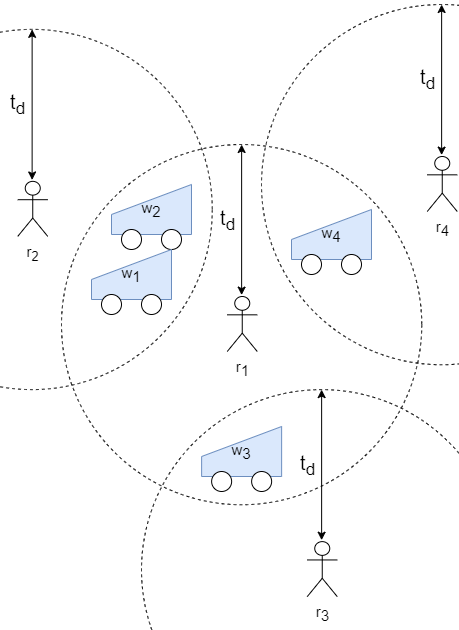
\includegraphics{FYP-LaTeX-Template/images/ota_hr2.png}
    \caption{Scenario for Highest Redundancy (destinations of requests not shown)}
    \label{fig:hr}
\end{figure}

Consider the scenario in Figure \ref{fig:hr}. Suppose the request $r_1$ is the first to arrive. We do not know yet that the other requests will are arriving. All workers $w_i$ are able to successfully fulfill $r_1$. The Greedy algorithm will assign  $w_1$, the Random algorithm will randomly assign a worker, and the Ranking algorithm will assign a worker based on the randomly assigned ranking done previously.

After the assignment to $r_1$ is made, the other requests, $r_2$, $r_3$ and $r_4$ arrive immediately. $r_2$ can be successfully fulfilled by $w_1$ or $w_2$; $r_3$ can be successfully fulfilled $w_3$ only; $r_4$ can be successfully fulfilled by $w_4$ only. 

Retrospectively, we should have assigned $w_1$ or $w_2$ to $r_1$. If either $w_3$ or $w_4$ was assigned, we would not be able to successfully assign a worker to $r_3$ or $r_4$ respectively.

Intuitively, we want to assign a worker that is close to other workers, such that a future request that could have been successfully assigned to that worker is likely to be able to be successfully assigned to the other workers that were close to that worker.

\subsection{Redundancy}
We could view the above notion to be similar to the concept of density, where we want to assign workers from worker dense areas. However, as workers are mobile, using the current location of other workers to calculate the density of workers around a particular worker may be inaccurate.

Instead, we use the next known location of workers to calculate the "density".
The \textit{next known location} of a worker would be its current location if it is currently idle and not fulfilling a request, otherwise, it would be the destination of the request the worker is currently fulfilling. Here, we consider "current" to be at the time at which the request arrives/is created, as the assignment is made immediately for each request in our problem.

We define an attribute known as \textit{redundancy} for a worker, given a parameter $k$, which represents the distance threshold. We define $redudancy(w,k)$ to be the number of workers whose next known location has a distance of at most $k$ from the next known location of $w$.

The concept of next known location and redundancy is illustrated in Figure \ref{fig:redundancy}. In this scenario, $w_1$, $w_3$, $w_4$ and $w_5$ are currently moving, and their next known locations are their destinations. $w_2$ and $w_6$ are idle, and their next known locations are their current locations.

To calculate the redundancy of $w_1$, we count the number of workers whose next known locations are within $k$ units from the next known location of $w_1$, which is $l$. $w_2$ and $w_6$ are currently idle and their next known locations are their current locations. Hence, $w_2$ is counted while $w_6$ is not. The next known locations of $w_3$, $w_4$ and $w_5$ are their destinations. Here $w_5$ is counted even though it is not currently within $k$ units of $l$. Even though $w_3$ and $w_4$ are currently in the vicinity of $l$, we do not count them as their next known locations are too far from $l$. Hence, $redundancy(w_1, k) = 2$, counting in $w_2$ and $w_5$.

\begin{figure}[h]
    \centering
    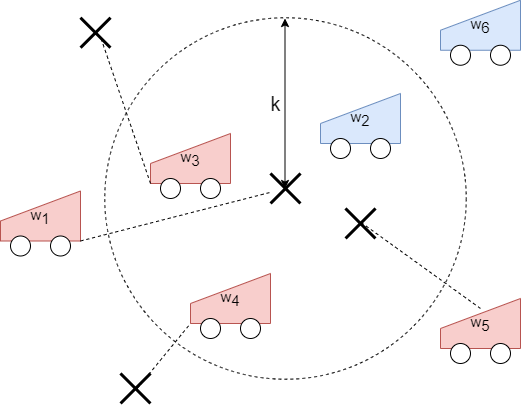
\includegraphics[scale = 0.6]{FYP-LaTeX-Template/images/ota_redundancy.png}
    \caption{Illustration of Redundancy}
    \label{fig:redundancy}
\end{figure}

\subsection{Algorithm Description}

In the highest redundancy algorithm, for each request, we first identify the feasible set of workers. If the feasible set of workers is not empty, we assign the worker with the highest redundancy with parameter $k$. Otherwise, we arbitrary assign a worker from the entire set of workers. \\

\begin{algorithm}[H]
\SetAlgoLined
\KwData{Set of workers $\W$, set of workers $\R$, maximum delay $t_d$, redundancy parameter $k$}
 \For{$r \in \R$}{
  construct feasible set $\W'$\;
  compute $redundancy(w, k)$  $\forall w \in \W'$\;
  \eIf{$|W'| \neq 0$}
  {assign arg$\max_{w \in \W'} redundancy(w, k)$ to $r$\;}
  {assign some $w \in \W$ to $r$\;}
 }
 \caption{Highest Redundancy}
\end{algorithm}

\subsection{Specific Details for Experiments}
In our experiments, we set the parameter $k = \frac{1}{2} t_d$. As we treat distance and time to be equivalently measured in our model (i.e. workers have unit velocity), setting $k$ to this value is equivalent to searching for workers whose next known location is within half the distance travelled during the maximum delay. Alternatively, the radius $k$ we use in Figure \ref{fig:redundancy} is set to be half that of the radius $t_d$ we use in Figure \ref{fig:hr}.

In addition, as per the Random and Ranking algorithms, if the feasible set is empty, we default to the Greedy algorithm in our experiments.


\chapter{Implementation, Methods and Dataset}
\label{ch:imp}
In this chapter, we discuss noteworthy details regarding the implementation of the model used for experimentation, the method we use in our experiments, and how request datasets are obtained for the experiments. The source code and real-world datasets are also available at \\ 
\url{https://github.com/weiyang13/ota}

\section{Implementation of Online Task Assignment}

As depicted in Figure \ref{fig:model}, we represent requests and workers as objects. The scheduler manages the workers, assigning them to requests. 

In the source code, the scheduler corresponds to the class \verb|Strategy| in \verb|ota_strategy.py|, and is inherited by subclasses representing each algorithm. To execute an instance of OTA, the method \verb|Strategy.run()| is called. \verb|Strategy.run()| is called with several parameters, including the initial set of workers, the initial set of requests, the maximum delay. The workers, requests, and their locations correspond respectively to the \verb|Worker|, \verb|Request|, and \verb|Location| classes in \verb|ota_lang.py|.

\begin{figure}[h]
    \centering
    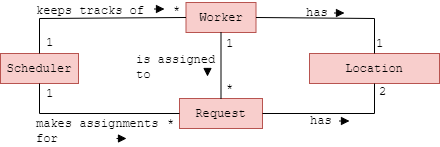
\includegraphics{FYP-LaTeX-Template/images/ota_modeloodm.png}
    \caption{Conceptual Class Diagram of OTA}
    \label{fig:model}
\end{figure}

\subsection{Interaction Between Workers and Requests}
Each \verb|Worker| object keeps track of the next known location, as well as the time at which it becomes idle. Each \verb|Request| object is composed of its start and end location, as well as the time of creation. 

When a \verb|Worker| is assigned to a \verb|Request|, it updates its next known location as well as the time at which it becomes idle using the calculations in Section \ref{prelim}. The distance metric used is the Euclidean distance between the coordinates stored in the \verb|Location| objects associated with the \verb|Worker| and \verb|Request| objects.

\subsection{Implementation of Algorithms}
While the \verb|Strategy| object has access to the entire set of requests when \verb|Strategy.run()| is called, within its implementation, the requests are assigned sequentially by the \verb|Strategy.assign()| method. Polymorphism is used for the \verb|Strategy.assign()| method, with the different subclasses of \verb|Strategy| (e.g. \verb|Greedy, Random|) having a different implementation based on the algorithm represented by the subclass.

While the implementation of \verb|Greedy| and \verb|Random| are straightforward, \verb|Ranking| requires some form of pre-processing to assign the randomly generated ranking. Also, while \verb|HighestRedundancy| can be naively implemented by directly computing redundancy for each assignment, this would result in a time complexity of $O(|\R||\W|^2)$, which would significantly increase the time taken for experiments.

To address these issues, a \verb|Strategy.initialize()| method is called before any assignment is made. For \verb|Ranking|, initialize allows for the rankings to be assigned first. The later assignments are based on the rankings made during this method.

For \verb|HighestRedundancy|, this allows for the use of dynamic programming to keep track of redundancy. An adjacency matrix for workers whose next known locations are close enough to each other (based on the parameter for highest redundancy) is constructed. The redundancy is calculated from the adjacency matrix for all workers and stored. In each call of \verb|Strategy.assign()|, the redundancy of each worker can be directly accessed. As the next known location of workers only changes upon assignment, we can update the adjacency matrix as well as the values of redundancy after each assignment. This reduces the time complexity of OTA under the Highest Redundancy algorithm to $O(|\R||\W|)$, assuming $|\R| \geq |\W|$, which is the same as the other algorithms.

\section{Experimental Methods}
In this section, we discuss the implementation of the experiments, as well as the environment under which the experiments are run.

\subsection{Implementation of Experiment Driver}
Figure \ref{fig:expdiag} shows the basic architecture used for the experiments. 

\begin{figure}[h]
    \centering
    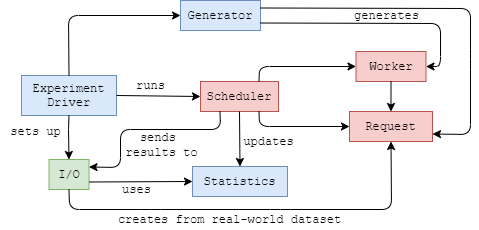
\includegraphics{FYP-LaTeX-Template/images/ota_expoodm.png}
    \caption{Architecture Diagram of Experimental Setup}
    \label{fig:expdiag}
\end{figure}

In the source code, some of the additional modules introduced are not implemented as classes, but the related functions are stored in separate files nonetheless. The generator, which generates synthetic request datasets, as well as the initial set of workers, are coded in \verb|ota_request_generator.py| and \verb|ota_worker_generator.py|. The statistics module is implemented as a class \verb|Statistics|, and keeps track of information about the OTA run such as the number of unsuccessfully assigned requests. 

The experiment driver is implemented in \verb|ota_experiment_driver.py|, and creates multiple \verb|Strategy| objects under different settings. In each experiment, the set of request is fixed: for synthetic request datasets, the number of requests and the distribution of requests; for real-world datasets, the input dataset file is fixed. All 4 algorithms are tested across a specified range of number of workers, and a specified range of maximum delay parameters. Each run is seeded so that the OTA sequence can be replicated if necessary.

The scheduler passes the results (in the form of a \verb|Statistics| object) to the I/O component in \verb|ota_io.py|. The \verb|Results| class in the I/O component is used to output the results of the experiment into a .csv file, detailing information about each OTA run, including the settings, the average delay, the maximum delay and the number of unsuccessfully assigned requests. A sample of the .csv file is shown in Figure \ref{fig:samplecsv}.

\begin{figure}
    \centering
    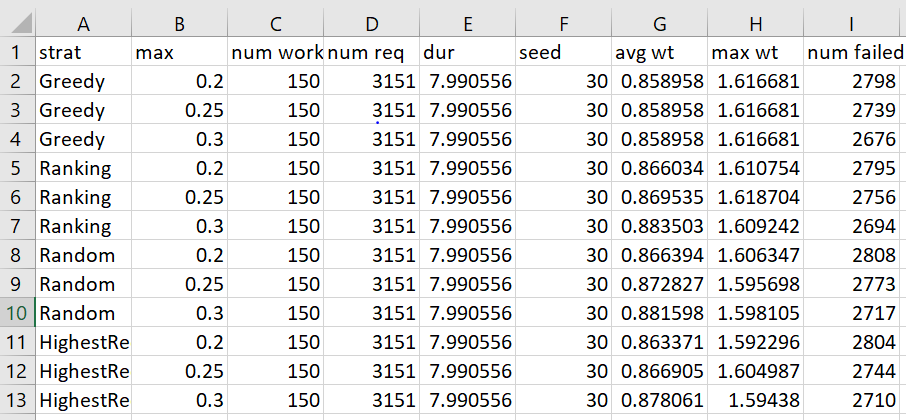
\includegraphics{FYP-LaTeX-Template/images/samplecsv.png}
    \caption{Sample of .csv Output from Experiments}
    \label{fig:samplecsv}
\end{figure}

Additionally, the I/O component has a function for reading input request data for the real-world dataset. We will further discuss the processing of the real-world dataset in the next section.

\subsection{Processing of Results}
The .csv results are manually inspected on Microsoft Excel to obtain the minimum number of workers to obtain a 99\% rate of success under each setting. This is tractable due to the relatively small scale of the experiments. This is then plotted on graphs using Microsoft Excel.

\subsection{Environment for Experiments}
The experiments were ran on the School of Computing (SoC) Compute Cluster. A Python 3.7 environment was created, with the required dependencies installed. Multiple experiments were run in parallel over multiple nodes from \verb|xcna| and \verb|xcnb| nodes. These nodes use CentOS 7.x, with a 2 x E5-2620 v2 CPU.


\section{Datasets}
In this section, we describe how the datasets for requests are obtained, and briefly discuss the generation of the initial set of workers as well. For the synthetic datasets, we will look at the implementation of \verb|ota_request_generation.py|, and \verb|ota_worker_generation.py|. For the real datasets, we will describe the procedure of obtaining the real datasets. At suitable points, we will also discuss the limitations of the datasets obtained.

\subsection{Synthetic Dataset (Experiment 1)}
\label{sec:exp1data}
\subsubsection{Generation of Requests}
A uniform temporal and spatial distribution was used for the generation of requests. That is, the time at which the request arrives/is created is uniformly generated within the specified period of time; the coordinates for the start and end locations of the request are also uniformly generated within the specified range of coordinates. Both the time of creation of request and the coordinates are stored as floating-point numbers. 

For Experiment 1, the duration over which the requests are created are within the range $[0, 100]$. The x-coordinates and y-coordinates are both uniformly distributed in the range $[0, 2]$. The choices made for these ranges were arbitrarily done as this was a pilot run before the real-world dataset was used.

\subsubsection{Generation of Workers}
The initial configuration of workers created is similar to that of the requests in Experiment 1. The initial locations were drawn from a uniform distribution in the same spatial dimensions as that of the requests. All workers start off idle, that is, all workers are available to fulfill a request at the start of the OTA run.

The use of the uniform distribution is applied for all 3 experiments, regardless of the distribution of request. 

\subsubsection{Limitations}
The datasets used for request lack the variety we see in the work of \cite{Tong} as only the uniform distribution is used. The indiscriminate use of the uniform distribution for the initial location of workers could possibly affect the minimum number of workers required. 

\subsection{Real-world Dataset (Experiment 2)}
\label{sec:exp2data}
For the second experiment, we used real-world taxi data from Brooklyn. This data is obtained from the New York City Taxi & Limousine Commission (NYC TLC), on \\ \url{https://bigquery.cloud.google.com/table/nyc-tlc:green.trips_2015}

The NYC TLC dataset in this source contains data on green taxi trips in the first 6 months of 2015. The dataset is comprehensive, containing many fields. In particular, we are interested in the time of pickup, the time of dropoff, as well as the longitude and latitude of pickup and dropoff. 

\subsubsection{Filtering by Location}
We do not take data from the whole of NYC due to the presence of water bodies, which would inevitably force the pickup and dropoff locations to be clustered at the land areas. Instead, we sectioned off a rectangular area of Brooklyn, as depicted in Figure \ref{fig:nyc} with the black lines.

\begin{figure}[h]
    \centering
    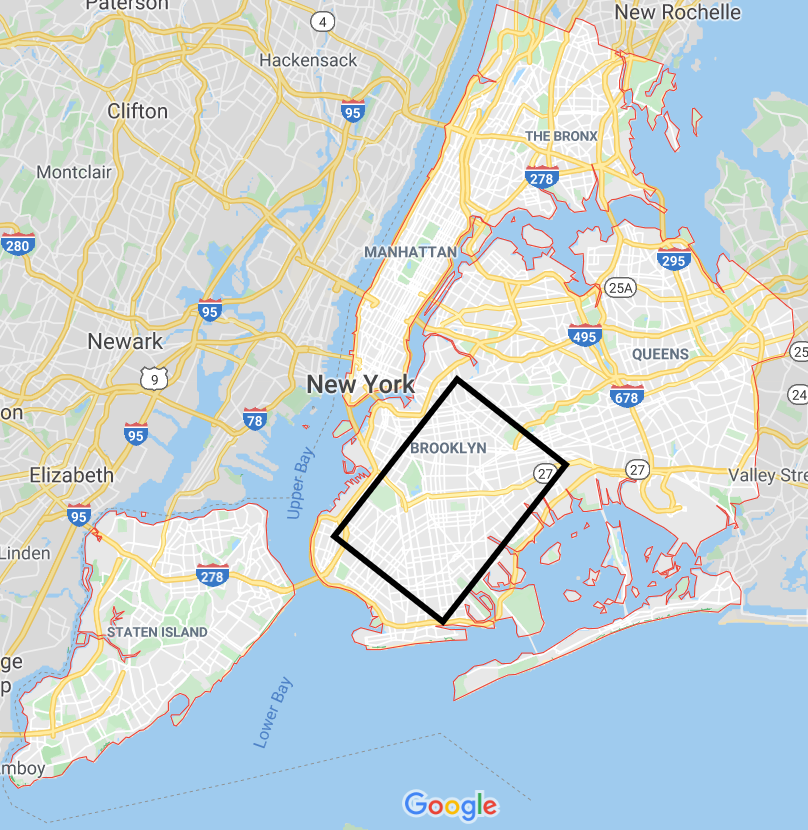
\includegraphics[scale=0.5]{FYP-LaTeX-Template/images/nyc.png}
    \caption{Selected Area in New York City (approximate)}
    \label{fig:nyc}
\end{figure}

We further manipulate the dataset by zeroing the longitude and latitude to the West-most corner of the selected region. Then, the modified longitude and latitude are rotated using a rotation matrix such that the selected area becomes a rectangle, as shown in \ref{fig:nycrotated}.

We select only data where both the pickup and dropoff occur within the selected area.

\begin{figure}
    \centering
    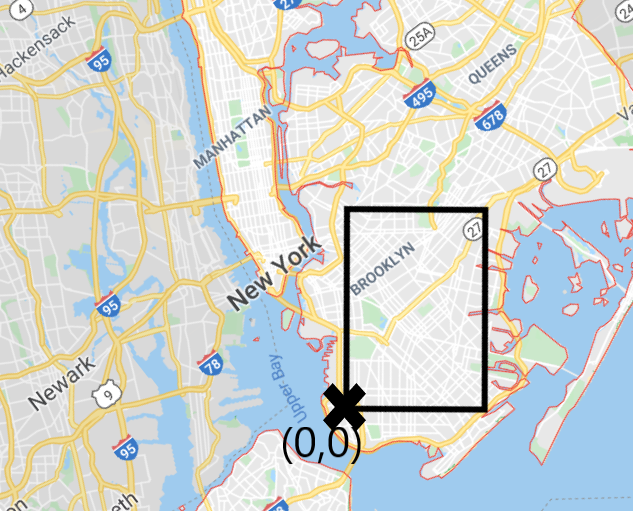
\includegraphics[scale=0.5]{FYP-LaTeX-Template/images/nyc_rotate.png}
    \caption{Rotation and Zeroing of Coordinates}
    \label{fig:nycrotated}
\end{figure}

\subsubsection{Filtering by Time}
In our problem, we assume that the same set of workers is used throughout the OTA run. To match our assumption, for each dataset we extract, we only take data from one night shift, that is, from 18:00 on one day to 02:00 on the next day, using America/New\_York time. 

For Experiment 2, the night shifts starting on 10 March, 14 April, 3 May, 20 May, 9 June and 21 June of 2015 were taken.

In addition, we noticed that there were data points with abnormally long and short time periods when we took the difference between the pickup and dropoff times. This could be due to a mistake on the part of the taxi driver in operating the system involved in recording the dataset. Accordingly, we placed additional filters to remove these outliers.

\subsubsection{Normalizing Velocity}
In our experiments, we assume that workers have unit velocity, that is they move 1 unit of distance in 1 unit of time. To normalize velocity, we first fix the scale of time such that 1 unit of time corresponds to 1 hour. Next, the dropoff time, pickup time, and start and end longitude and latitude are used to calculate the velocity of the taxi driver in each request. The average velocity is taken for all data points in the selected area in the 2015 dataset. The x and y coordinates obtained after rotation are then scaled accordingly such that a unit velocity is obtained.


\subsubsection{SQL Queries}
The methods described above were performed in 7 SQL queries to the BigQuery dataset. The first query was used to determine the average velocity over the entire 2015 dataset within the selected area. Each of the second to seventh SQL queries were used to obtain the 6 datasets for each shift. The first SQL query, \verb|avgvelocityquery.sql|, and third SQL query, \verb|brooklyndataquery140415.sql|, are found in the \verb|dataset/brooklyn| folder. The other SQL queries are a simple manipulation of the third SQL query, by changing the variables storing the start and end times of the shift.

The query results are downloaded as a .csv file to be used as inputs. The fields in the .csv file are the pickup time, and the transformed coordinates of the start and end location of each request. The number of requests for each shift is shown in Table \ref{tab:numreq} 
\begin{table}[h]
    \centering
    \begin{tabular}{|c|c|}
        \hline
         \textbf{Date of Shift Start} & \textbf{Number of Requests}\\
         \hline
         10 March 2015 & 3177 \\
         \hline
         14 April 2015 & 2577 \\
         \hline
         3 May 2015 & 2903 \\
         \hline
         20 May 2015 & 3946 \\
         \hline
         9 June 2015 & 2964 \\
         \hline
         21 June 2015 & 3151 \\
        \hline
    \end{tabular}
    \caption{Number of Requests in Shifts from Brooklyn Data}
    \label{tab:numreq}
\end{table}

\subsubsection{Limitations}
A major limitation of the real-world data use is its applicability to our problem. Even though a contiguous area of land is used, the underlying transport structure for the data is still a traffic network, which is badly captured by the Cartesian plane model used.

\subsection{Adjusted Synthetic Dataset (Experiment 3)}
\label{sec:exp3data}
Following the results in Experiment 2, which will be detailed in Chapter \ref{ch:exp}, we made adjustments to the synthetic dataset such that the dimensions, duration, and number of requests is similar to that of the real-world datasets used. Specifically, the x-coordinates are drawn from the range [0, 0.603]; the y-coordinates are drawn from the range [0, 0.979]; the time of request creation is drawn from the range [0, 8]; the number of requests used in each OTA run is 2500, 3000 or 3500.

In addition, a simple analysis of the spatial and temporal distributions of the real-world dataset from 9 June 2015 was taken. These distributions were then used to generate two new types of synthetic data, the Brooklyn Spatial Distribution and Brooklyn Temporal Distribution

\subsubsection{Brooklyn Spatial Distribution}
To analyse the spatial distribution of requests, the coordinates of the start and end locations were each divided into sextiles, and the number of requests were counted. A density plot of the results are shown in \ref{fig:brooklyn_space}. 

\begin{figure}[h]
    \centering
    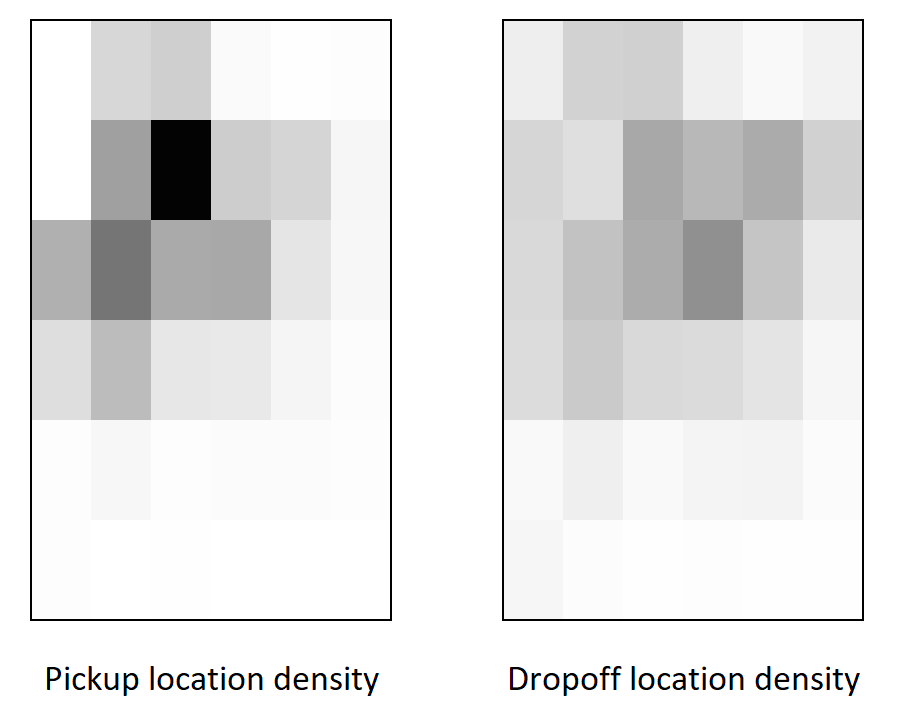
\includegraphics[scale=0.5]{FYP-LaTeX-Template/images/ota_brooklynspace.png}
    \caption{Spatial Distribution of Requests in Brooklyn (9 June shift)}
    \label{fig:brooklyn_space}
\end{figure}

We observe that the start and end locations are concentrated in the middle-top region of the selected area. The distribution for the pickup locations is more concentrated, while that of the dropoff locations is more diffuse. We took the marginal distributions for each coordinate to generate the new set of requests. The marginal distributions are used independently, and the temporal distribution used is uniform.

\subsubsection{Brooklyn Temporal Distribution}

To analyse the temporal distribution of requests, we count the number of requests in each hour. A bar graph of the results is shown in Figure \ref{fig:brooklyn_space}. 

\begin{figure}[h]
    \centering
    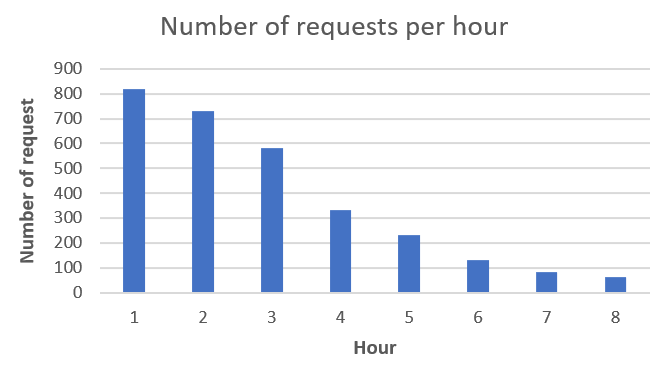
\includegraphics[scale=0.9]{FYP-LaTeX-Template/images/ota_brooklyntime.png}
    \caption{Temporal Distribution of Requests in Brooklyn (9 June shift)}
    \label{fig:brooklyn_time}
\end{figure}

We observe that the number of requests per hour drop as time passes. From here, we use the proportion of requests in each hour to create a temporal distributions. Requests were generated using this temporal distribution, as well as a uniform spatial distribution.

\subsubsection{Limitations}
A major limitation is the independence assumptions used to capture the spatial distribution of the requests in Brooklyn. The independence of x- and y-coordinates causes inaccuracies in capturing the distribution. More significantly, the start and end locations are generated independently. Furthermore, the separation of spatial and temporal distribution may cause interaction effects not to be captured.

In general, more fine-grained estimations of the temporal and spatial distributions could also be used.


\chapter{Experiments and Analysis}
\label{ch:exp}
In this chapter, we discuss representative results from the experiments conducted and the insights we gain from it. The tables depicting the minimum fleet sizes can be found in Section \ref{ch:appendixtables} of the Appendix. Table \ref{tab:expsummary} recaps and summarizes the settings used for each experiment.
\newline

\begin{table}[h!]
    \centering
    \begin{tabular}{|c||c|c|c|}
    \hline
         Experiment &  1 & 2 & 3\\
         \hline \hline
         Request  & Uniform & Real-World & Uniform, Brooklyn Spatial \\ Distribution&&&or Brooklyn Temporal\\
         \hline
         Number of Requests & Varies from 600-1400 & By dataset & 2500, 3000 or 3500 \\
         \hline
         Space & [0,0] to [2,2] & [0,0] to [0.603,0.979] & [0,0] to [0.603,0.979] \\
         \hline
         Time & 0 to 100 & 0 to 8 & 0 to 8 \\
         \hline
         Max Delay & Varies from 0.1-0.45 & 0.2, 0.25 or 0.30& 0.2, 0.25 or 0.30\\
         \hline
         Number of & Up to 300,  & Up to 500,  & Up to 500,  \\ Workers&precise to 10&precise to 5&precise to 5 \\
         \hline
         Algorithms Tested & All & All & All \\
         \hline
    \end{tabular}
    \caption{Summary of Experimental Settings}
    \label{tab:expsummary}
\end{table}

\section{Experiment 1: Preliminary Experiment}
In Experiment 1, we used uniformly generated requests as detailed in Section \ref{sec:exp1data}. This experiment is a preliminary one done with the settings in Table \ref{tab:expsummary} set arbitrarily.

In the conduct of this experiment, three readings of the number of requests that were unsuccessful were obtained for every number of worker tested using different seeds. The average was then used to find the minimum fleet size where at least 99\% of requests were successful. 

\begin{figure}[h]
    \centering
    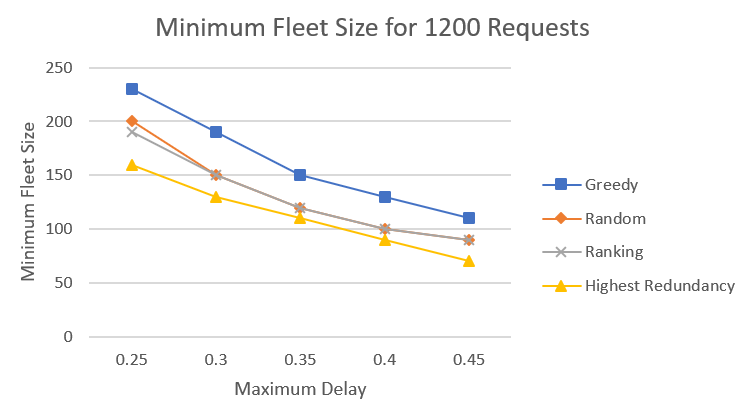
\includegraphics{FYP-LaTeX-Template/images/ota_exp1_1200.png}
    \caption{Effect of Algorithm and Maximum Delay on Minimum Fleet Size}
    \label{fig:exp1graphdelay}
\end{figure}

Figure \ref{fig:exp1graphdelay} shows how the minimum fleet size changes with maximum delay when there are 1200 requests. We observe that there is a general decrease in minimum fleet size as maximum delay increases. In addition, the Greedy algorithm shows the worst performance, consistently having the greatest minimum fleet size, whereas the Highest Redundancy algorithm has the smallest minimum fleet size. The Random and Ranking algorithm produce similar minimum fleet sizes. These trends are also observed when the number of requests is set to other values.

\begin{figure}
    \centering
    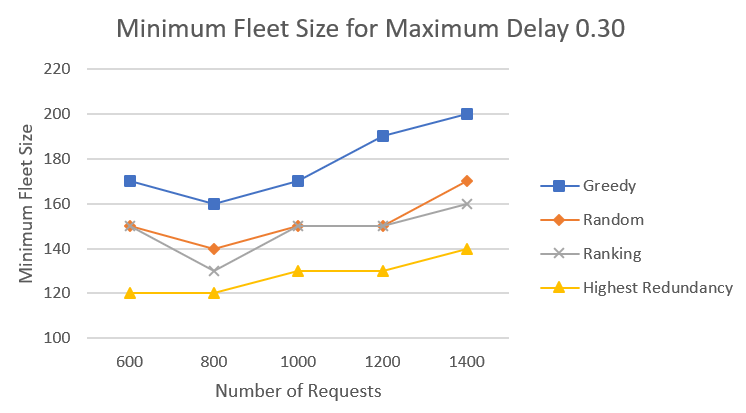
\includegraphics{FYP-LaTeX-Template/images/ota_exp1_030.png}
    \caption{Effect of Algorithm and Number of Requests on Minimum Fleet Size}
    \label{fig:exp1graphnumreq}
\end{figure}

Figure \ref{fig:exp1graphnumreq} shows how the minimum fleet size changes with the number of requests when the maximum delay is set at 0.30. There is a general increase in minimum fleet size as number of requests increases, but this trend is less consistent. The same trend is observed when comparing the four algorithms. These trends are also observed when the maximum delay is set to other values, with some outliers as well.

It was unexpected that the Random and Ranking algorithm performed better than the Greedy algorithm. The similarity between the Random and Ranking algorithm was somewhat expected as in effect, both algorithms pick a random worker from the feasible set. The better performance of the Highest Redundancy algorithm shows that the heuristic we developed (assigning workers from worker dense area) was successful.

\section{Experiment 2: Brooklyn Taxi Shifts}
In Experiment 2, we used real-world data as detailed in Section \ref{sec:exp2data}. The settings for this experiment can be found in Table \ref{tab:expsummary} above.

Unlike Experiment 1, only one reading of the number of requests that were unsuccessful was obtained for every number of worker tested. This single reading was used to find the minimum fleet size where at least 99\% of requests were successful. 

The range of number of workers (up to 500) was selected so that average number of request each worker can fulfill is sensible for an 8 hour period. The range of maximum delay was chosen with consideration of the equivalent time in the real-world setting. Specifically, the maximum delays used in this experiment, 0.25, 0.3 and 0.35, correspond to 15 minutes, 18 minutes, and 21 minutes of delay.

In light of the relatively realistic setting, the results were dismal. At the max delay of 0.20, the Greedy and Ranking algorithms had a minimum fleet size above 500 for all shifts, and the Random and Highest Redundancy algorithms had a minimum fleet size above 500 for the shifts that had more requests.

\begin{figure}[h]
    \centering
    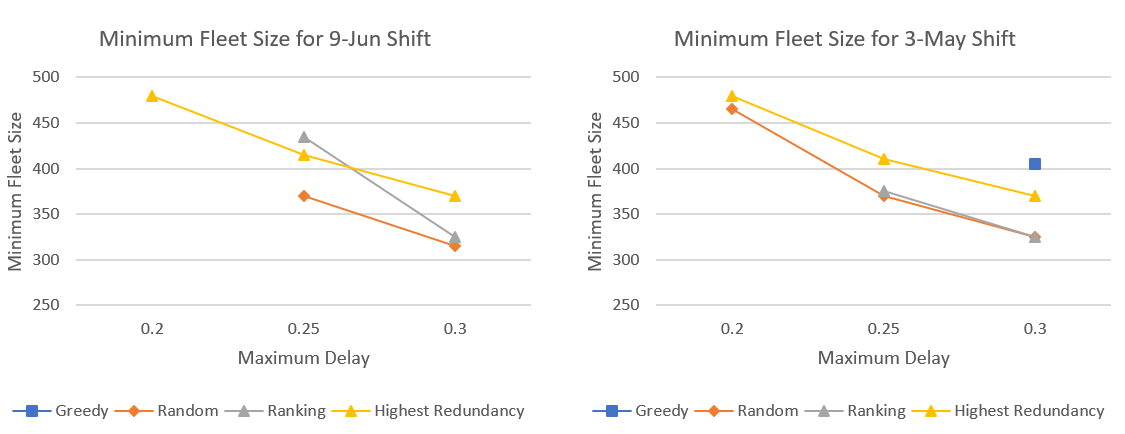
\includegraphics[scale=0.80]{FYP-LaTeX-Template/images/ota_exp2_1.png}
    \caption{Minimum Fleet Size for Brooklyn Shifts}
    \label{fig:exp2_multi}
\end{figure}

There were several unexpected trends observed as well. Figure \ref{fig:exp2_multi} depicts the minimum fleet size results for two shifts. The missing data points correspond to having a minimum fleet size above 500. From Figure \ref{fig:exp2_multi}, we see that Random generally produces the smallest minimum fleet size, except sometimes when the maximum delay is at 0.20, where the Highest Redundancy has a smaller fleet size. This is in contrast to Experiment 1, where the Highest Redundancy algorithm shows the best performance.

\begin{figure}[h]
    \centering
    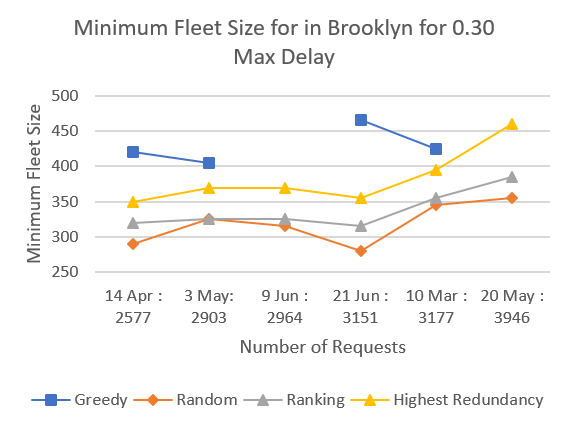
\includegraphics[scale=0.8]{FYP-LaTeX-Template/images/ota_exp2_030.png}
    \caption{Minimum Fleet Size for Brooklyn Shifts at Max Delay 0.30}
    \label{fig:exp2_delay}
\end{figure}

Furthermore, as the maximum delay increases to 0.30, the Ranking algorithm performs better than the Highest Redundancy algorithm, as seen in Figure \ref{fig:exp2_delay}. The divergence between the Random and Ranking algorithms, which in Experiment 1 shows similar performance, becomes clearer in Figure \ref{fig:exp2_delay} as well. What conforms with our expectations is the performance of the Greedy algorithm, which is worse than the other three algorithms.

\section{Experiment 3: Decomposing the Differences Between Datasets}
To shed light on why there are differences in the trends observed in Experiments 1 and 2, we analyse the differences between the settings of these two experiments. Firstly, the range of space and time, as well as the number of requests are different in the two experiments. Secondly, the distribution of requests across the area in Experiment 2 is not uniform. Thirdly, the distribution of requests across time in Experiment 2 is not uniform.

With the multitude of differences observed, we chose to conduct Experiment 3 to decompose these differences by adjusting the synthetic data. We first use uniformly generated requests with adjusted time and space dimensions, and a comparable number of requests, to observe the effect of these factors. 

This serves as a baseline to use the Brooklyn spatial and Brooklyn temporal distributions, which respectively act as a substitute for the spatial distribution and temporal distribution for the requests in Brooklyn. This allows us to separately analyse the effects of these two differences.

The details of how the synthetic data was adjusted is described in Section \ref{sec:exp2data}. Again, the settings for this experiment can be found in Table \ref{tab:expsummary} above. 

Like Experiment 2, only one reading of the number of requests that were unsuccessful was obtained for every number of worker tested. This single reading was used to find the minimum fleet size where at least 99\% of requests were successful. 

\subsection{Uniform Distribution}
From Figure \ref{fig:exp3_unif}, we see that for 2500 requests, Highest Redundancy remains as the best performing algorithm, as in Experiment 1.

\begin{figure}[h]
    \centering
    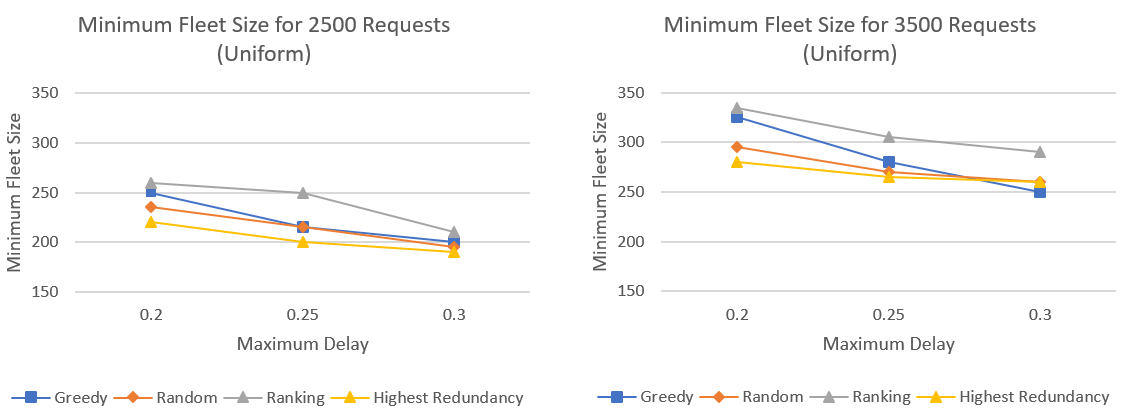
\includegraphics[scale=0.8]{FYP-LaTeX-Template/images/ota_exp3_unif.png}
    \caption{Minimum Fleet Size for Uniform Distribution at 2500 and 3500 Requests}
    \label{fig:exp3_unif}
\end{figure}

However, contrary to Experiment 1, there is a significant divergence between the performance of the Ranking and Random algorithm, even though a Uniform distribution is used for request generation. Furthermore, the Greedy algorithm outperforms the Ranking algorithm, and even outperforms the Random and Highest Redundancy algorithms when the experiment is run with 3500 requests.


\subsection{Brooklyn Spatial Distribution}
With reference to Figure \ref{exp3_peaks}, we observe that the Greedy algorithm performs poorly under the Brooklyn Spatial Distribution. The divergence between Ranking and Random algorithms remain, with the Random algorithm consistently performing better than the Ranking algorithm. The Highest Redundancy algorithm has a relatively good performance for a maximum delay of 0.2, but it is outperformed by both the Random and Ranking algorithm when the max delay increases.

\begin{figure}[h]
    \centering
    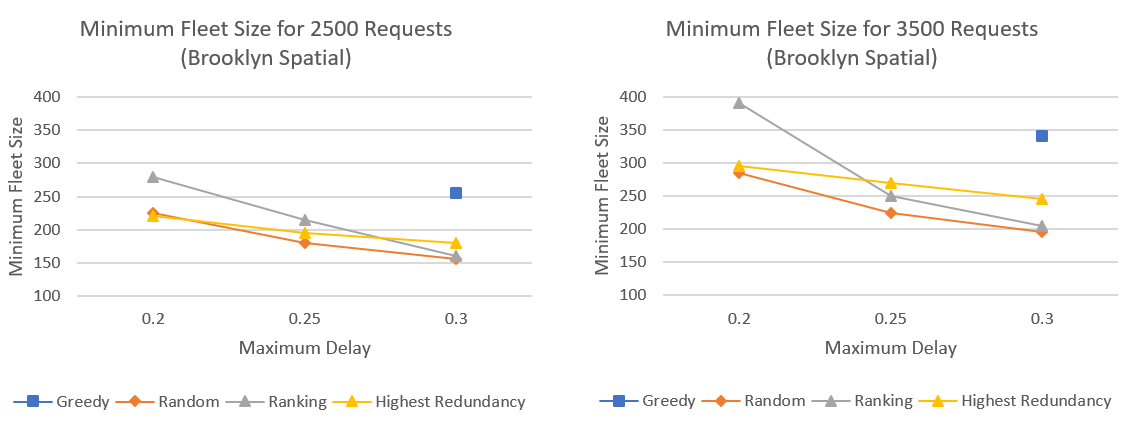
\includegraphics[scale=0.8]{FYP-LaTeX-Template/images/ota_exp3_peaks.png}
    \caption{Minimum Fleet Size for Brooklyn Spatial Distribution at 2500 and 3500 Requests}
    \label{fig:exp3_peaks}
\end{figure}


\subsection{Brooklyn Temporal Distribution}
We see an interesting trend in Figure \ref{fig:exp3_peakt}, where the Greedy algorithm becomes the best performing algorithm, more so than in the uniform distribution. The performance of the other 3 algorithms are similar, with the Highest Redundancy algorithm marginally performing better than the other 2 algorithms.

\begin{figure}[h]
    \centering
    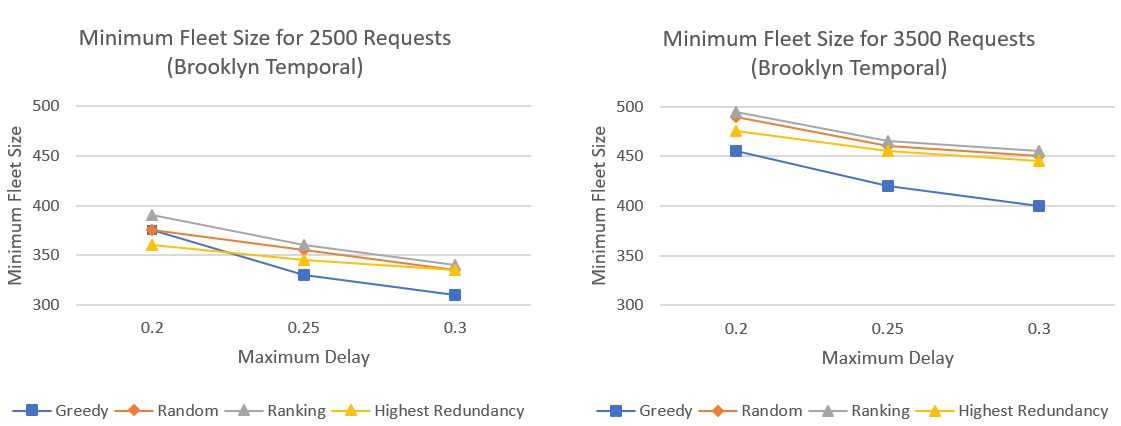
\includegraphics[scale=0.8]{FYP-LaTeX-Template/images/ota_exp3_peakt.png}
    \caption{Minimum Fleet Size for Brooklyn Temporal Distribution at 2500 and 3500 Requests}
    \label{fig:exp3_peakt}
\end{figure}

\newpage
\subsection{Comparison}
For each setting, a comparison was done between the 3 distributions, as well as with the results from a suitable dataset (of comparable number of requests) from Experiment 2.

In Figure \ref{fig:exp3_integrated} we show a bar chart that illustrates the differences between these 4 distributions for each of the algorithms. Note that the missing bar for the Greedy algorithm is due to a minimum fleet size that is out of range for the experiment.

\begin{figure}[h]
    \centering
    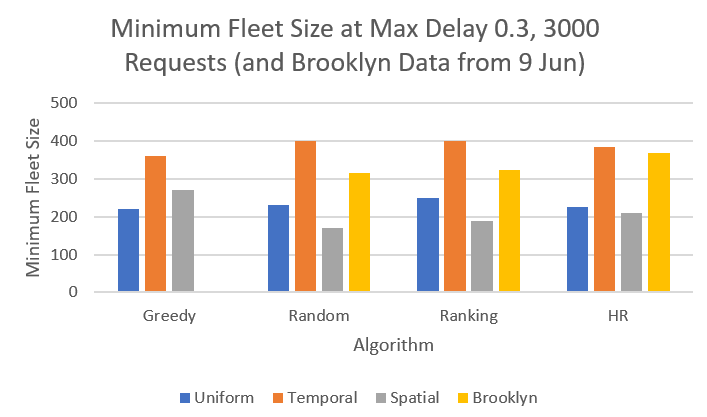
\includegraphics{FYP-LaTeX-Template/images/ota_exp3_integrated.png}
    \caption{Comparison of Different Distributions}
    \label{fig:exp3_integrated}
\end{figure}

When we compare the Uniform distribution and the Brooklyn Temporal distribution, there is always an increase in the minimum fleet size. This increase is less pronounced for the Greedy algorithm.

Interestingly, when we compare the Uniform distribution and the Brooklyn Spatial, the Greedy algorithm shows an increase in the minimum fleet size. On the other hand, the Random shows a consistent decrease in minimum fleet size. The Ranking algorithm generally shows a smaller decrease in the minimum fleet size, except for when the maximum delay is 0.2, for which it shows an increase in minimum fleet size. For the Highest Redundancy algorithm, the minimum fleet size remains at around the same level.

From Figure \ref{fig:exp3_integrated}, it seems that the minimum fleet size for the Brooklyn data is lower than that of the Brooklyn Temporal Distribution for the Random, Ranking and Highest Redundancy Algorithms, suggesting a dampening effect due to the spatial distribution. This observation is consistent for the Random algorithm under a maximum delay of 0.25 or 0.3, but is not as consistent for the Ranking or Highest Redundancy algorithms.

\section{Discussion}
While the difference between the trends in Experiment 1 and Experiment 3 (for the Uniform distribution) is stark, this is likely due to the vastly different density of requests over time, as the number of requests in Experiment 3 was much greater, and over a shorter period of time.

The relatively better performance of the Greedy algorithm in Experiment 3 under the Uniform distribution suggests that it performs well under high request density. This is supported by the results of the Brooklyn Temporal Distribution. The Brooklyn Temporal Distribution starts off with a high density of request, which decreases as time passes. It is likely that most of the unsuccessfully fulfilled requests occur during the early busy period. In essence, this distribution increases the density of requests significantly for a short period of time. The markedly better performance of the Greedy algorithm further shows its relative effectiveness in high request density situations.

Consequently, there is a need to increase the scale of the study to better understand the effect of request density. This also applies to maximum delay. In our experiments, the maximum delay of 0.2 seems to go below a threshold required for good performance.

Another fascinating observation is the different behaviour of the algorithms under the Brooklyn Spatial Distribution. As the distribution of requests in Brooklyn is largely concentrated around the middle-top area, this could have the same effect as shrinking the area in which we perform the task assignment, which helps to improve performance. Such a perspective could help explain why the Random algorithm performs better with this distribution.

As for the worse performance of the Greedy algorithm, this could be due to the 'bias' of the algorithm in choosing workers close to the start location of the request. Together with the fact that the distribution of the end locations is concentrated in the same region as the start locations, this essentially causes the algorithm to restrict itself to only use a small subset of workers to complete requests.

The Highest Redundancy algorithm, on the other hand, does not see a boost in performance as compared to the Random algorithm. This could be due to a similar bias as in the Greedy algorithm. The use of redundancy has dual effects: it tends to pick workers from areas that are less popular starting location for requests, since the workers who end up at these locations would accumulate; it also tends to pick workers from areas which are popular as destinations for requests, since workers would accumulate there. As the destination, or end location, of requests is concentrated in the same region as the start location of requests, this creates the same problem as in the Greedy algorithm - where the workers outside of this 'hotspot' are more likely to be ignored.

A possible modification to the Highest Redundancy algorithm to improve its performance would be to take into account the distribution of request. We could weight the redundancy measure with the probability of a request starting in the associated region.

A last observation is the unexpected divergence in performance between the Ranking and Random algorithms. While the same concept of 'bias' can be used as an intuitive explanation in the case of the Brooklyn Spatial Distribution, it is more difficult to explain why this divergence still exists in the Uniform distribution for Experiment 3.

\chapter{Conclusion}
\label{ch:con}
\section{Contributions}
In this project, we described algorithms for the minimum fleet problem based on algorithms used in other problems. In particular, we adapted the underlying idea of the G-llep algorithm from \cite{kazemi} to devise the Highest Redundancy algorithm.

We have also established methods used to study the minimum fleet problem, and online task assignment in general. Using these methods, we analysed the effect of spatial and temporal distributions of requests on the performance of various algorithms in the minimum fleet problem. We obtain the following findings:

\begin{itemize}
    \item The Greedy algorithm performs well with high request density, but not under the settings studied where the spatial distribution of requests is not uniform. 
    \item The Ranking algorithm generally leads to a higher minimum fleet size compared to the Random algorithm in most of the settings studied, and is thus not ideal.
    \item The Highest Redundancy algorithm shows some promise, but does not perform as well as the Random and Ranking algorithms when the spatial distribution is not uniform.
\end{itemize}

While our results point to the Random algorithm being most suited for a real-world scenario for the minimum fleet problem, we suggest modifications of the Highest Redundancy algorithm to improve its performance as well. 

\section{Future Work}

\subsubsection{Modifications to Workers}
The experiments all start with the workers being uniformly distributed across space. The initial distribution can be modified to better fit the set of requests.

In addition, the assumptions made in this problem can be altered. For example, we can allow workers to move when idle, which would better depict reality. This allows us to redirect workers in areas with low demand to areas with high demand. It also allows us to incorporate stochasticity in the location of workers when studying this problem.

\subsubsection{Modifications to Highest Redundancy Algorithm}
As highlighted in our discussion, the performance of the Highest Redundancy algorithm could possibly be improved by taking into consideration the spatial distribution of requests when calculating redundancy. Furthermore, more experimentation can be done in altering the parameter used in calculating redundancy (that is, the radius in which we count workers who will be nearby).

\subsubsection{Tradeoff with Average Delay}
While average delay is not considered at all in our problem, it is often used as a performance metric in other studies. Across all three experiments, we observe 2 general trends:
\begin{itemize}
    \item Fixing the number of workers and the number of requests, the Greedy algorithm
    \item As the maximum delay permitted increases, the average delay for the Random, Ranking, and Highest Redundancy algorithms increases. 
\end{itemize}
The first trend is expected as the Greedy algorithm seeks to minimize average delay. The second trend is also expected, as increasing the maximum delay allows the stated algorithms to pick workers that are further away.

Further investigation can be done to analyse the impact of these algorithms on the average delay. This can also involve studying algorithms that are partly "Greedy", in that the selection of a worker first occurs in a smaller feasible set, and the entire feasible set is only considered when this smaller feasible set is empty.

\subsubsection{Graph Model of Locations}
The use of a Cartesian plane as a model for OTA may not be applicable to real-world scenarios. The algorithms studied could be modified and applied to a model where a network is used to measure distance or cost.

\bibliographystyle{socreport}
\bibliography{socreport}

\appendix
\chapter{Tables of Results}
\label{ch:appendixtables}
This section documents the minimum fleet size (to attain 99\% success) obtained for Experiment 1-3. Tables \ref{tab:exp1_600} to \ref{tab:exp1_1400} are for Experiment 1; Tables \ref{tab:exp2_1003} to \ref{tab:exp2_2106} are for Experiment 2; Tables \ref{tab:exp3_unif2500} to \ref{tab:exp3_peakt3500} are for Experiment 3.

For experiment 1, The range of fleet size tested is up to 300, with a precision of 10 (tested in increments of 10). The range of maximum delay parameter is [0.1, 0.15, 0.2, 0.25, 0.3, 0.35, 0.4, 0.45]. The values for 0.1 and 0.15 are omitted because they are out of range. Experiment 1 consists of Uniformly distributed requests in a 2x2 Cartesian Plane

For Experiments 2 and 3, the range of fleet size tested is up to 500, with a precision of 5 (tested in increments of 5). The range of maximum delay parameter is [0.2, 0.25, 0.3]. Experiments 2 and 3 are done on a  0.603x0.979 Cartesian Plane

For all tables, Values that are out of range will be denoted with a (*).

\begin{table}[h!]
    \centering
    \begin{tabular}{|c|c|c|c|c|c|c|}
        \hline
         & \multicolumn{6}{|c|}{\textbf{MAX DELAY}}\\
         \hline
         \textbf{ALGORITHM} & \textbf{0.2} & \textbf{0.25}& \textbf{0.3}& \textbf{0.35}& \textbf{0.4}& \textbf{0.45}\\
         \hline \hline
         \textbf{Greedy} & (*) & 250 & 170 & 140 & 110 & 100\\
         \hline
         \textbf{Random} & 280 & 210 & 150 & 120 & 110 & 80 \\
         \hline
         \textbf{Ranking} & 260 & 190 & 150 & 120 & 100 & 90 \\
         \hline
         \textbf{Highest Redundancy} & 230 & 160 & 120 & 100 & 80 & 60 \\
        \hline
    \end{tabular}
    \caption{Minimum Fleet Size for 600 Requests in Uniform Distribution}
    \label{tab:exp1_600}
\end{table}

\begin{table}[h!]
    \centering
    \begin{tabular}{|c|c|c|c|c|c|c|}
        \hline
         & \multicolumn{6}{|c|}{\textbf{MAX DELAY}}\\
         \hline
         \textbf{ALGORITHM} & \textbf{0.2} & \textbf{0.25}& \textbf{0.3}& \textbf{0.35}& \textbf{0.4}& \textbf{0.45}\\
         \hline \hline
         \textbf{Greedy} & 300 & 220 & 160 & 130 & 110 & 90\\
         \hline
         \textbf{Random} & 270 & 170 & 140 & 100 & 100 & 70 \\
         \hline
         \textbf{Ranking} & 270 & 170 & 130 & 100 & 100 & 80 \\
         \hline
         \textbf{Highest Redundancy} & 220 & 140 & 120 & 90 & 70 & 60 \\
        \hline
    \end{tabular}
    \caption{Minimum Fleet Size for 800 Requests in Uniform Distribution}
    \label{tab:exp1_800}
\end{table}

\begin{table}[h!]
    \centering
    \begin{tabular}{|c|c|c|c|c|c|c|}
        \hline
         & \multicolumn{6}{|c|}{\textbf{MAX DELAY}}\\
         \hline
         \textbf{ALGORITHM} & \textbf{0.2} & \textbf{0.25}& \textbf{0.3}& \textbf{0.35}& \textbf{0.4}& \textbf{0.45}\\
         \hline \hline
         \textbf{Greedy} & (*) & 200 & 170 & 130 & 120 & 100\\
         \hline
         \textbf{Random} & 280 & 190 & 150 & 120 & 100 & 80 \\
         \hline
         \textbf{Ranking} & 280 & 190 & 150 & 140 & 100 & 90 \\
         \hline
         \textbf{Highest Redundancy} & 230 & 160 & 130 & 100 & 80 & 70 \\
        \hline
    \end{tabular}
    \caption{Minimum Fleet Size for 1000 Requests in Uniform Distribution}
    \label{tab:exp1_1000}
\end{table}

\begin{table}[h!]
    \centering
    \begin{tabular}{|c|c|c|c|c|c|c|}
        \hline
         & \multicolumn{6}{|c|}{\textbf{MAX DELAY}}\\
         \hline
         \textbf{ALGORITHM} & \textbf{0.2} & \textbf{0.25}& \textbf{0.3}& \textbf{0.35}& \textbf{0.4}& \textbf{0.45}\\
         \hline \hline
         \textbf{Greedy} & (*) & 230 & 190 & 150 & 130 & 110\\
         \hline
         \textbf{Random} & 260 & 200 & 150 & 120 & 110 & 90 \\
         \hline
         \textbf{Ranking} & 270 & 190 & 150 & 120 & 100 & 90 \\
         \hline
         \textbf{Highest Redundancy} & 220 & 160 & 130 & 110 & 90 & 70 \\
        \hline
    \end{tabular}
    \caption{Minimum Fleet Size for 1200 Requests in Uniform Distribution}
    \label{tab:exp1_1200}
\end{table}

\begin{table}[h!]
    \centering
    \begin{tabular}{|c|c|c|c|c|c|c|}
        \hline
         & \multicolumn{6}{|c|}{\textbf{MAX DELAY}}\\
         \hline
         \textbf{ALGORITHM} & \textbf{0.2} & \textbf{0.25}& \textbf{0.3}& \textbf{0.35}& \textbf{0.4}& \textbf{0.45}\\
         \hline \hline
         \textbf{Greedy} & (*) & 260 & 200 & 160 & 140 & 120\\
         \hline
         \textbf{Random} & 300 & 200 & 170 & 140 & 110 & 100 \\
         \hline
         \textbf{Ranking} & (*) & 210 & 160 & 140 & 140 & 110 \\
         \hline
         \textbf{Highest Redundancy} & 240 & 180 & 140 & 110 & 90 & 80 \\
        \hline
    \end{tabular}
    \caption{Minimum Fleet Size for 1400 Requests in Uniform Distribution}
    \label{tab:exp1_1400}
\end{table}



\begin{table}[h!]
    \centering
    \begin{tabular}{|c|c|c|c|}
        \hline
         & \multicolumn{3}{|c|}{\textbf{MAX DELAY}}\\
         \hline
         \textbf{ALGORITHM} & \textbf{0.2} & \textbf{0.25}& \textbf{0.3}\\
         \hline \hline
         \textbf{Greedy} & (*) & (*) & 425\\
         \hline
         \textbf{Random} & (*) & 405 & 345\\
         \hline
         \textbf{Ranking} & (*) & 415 & 355\\
         \hline
         \textbf{Highest Redundancy} & (*) & 460 & 395\\
        \hline
    \end{tabular}
    \caption{Minimum Fleet Size for Brooklyn Shift on 10 Mar (3177 requests)}
    \label{tab:exp2_1003}
\end{table}

\begin{table}[h!]
    \centering
    \begin{tabular}{|c|c|c|c|}
        \hline
         & \multicolumn{3}{|c|}{\textbf{MAX DELAY}}\\
         \hline
         \textbf{ALGORITHM} & \textbf{0.2} & \textbf{0.25}& \textbf{0.3}\\
         \hline \hline
         \textbf{Greedy} & (*) & (*) & 420\\
         \hline
         \textbf{Random} & 455 & 345 & 290\\
         \hline
         \textbf{Ranking} & (*) & 400 & 320\\
         \hline
         \textbf{Highest Redundancy} & 455 & 395 & 350\\
        \hline
    \end{tabular}
    \caption{Minimum Fleet Size for Brooklyn Shift on 14 Apr (2577 requests)}
    \label{tab:exp2_1404}
\end{table}

\begin{table}[h!]
    \centering
    \begin{tabular}{|c|c|c|c|}
        \hline
         & \multicolumn{3}{|c|}{\textbf{MAX DELAY}}\\
         \hline
         \textbf{ALGORITHM} & \textbf{0.2} & \textbf{0.25}& \textbf{0.3}\\
         \hline \hline
         \textbf{Greedy} & (*) & (*) & 405\\
         \hline
         \textbf{Random} & 465 & 370 & 325\\
         \hline
         \textbf{Ranking} & (*) & 375 & 325\\
         \hline
         \textbf{Highest Redundancy} & 480 & 410 & 370\\
        \hline
    \end{tabular}
    \caption{Minimum Fleet Size for Brooklyn Shift on 3 May (2903 requests)}
    \label{tab:exp2_0305}
\end{table}

\begin{table}[h!]
    \centering
    \begin{tabular}{|c|c|c|c|}
        \hline
         & \multicolumn{3}{|c|}{\textbf{MAX DELAY}}\\
         \hline
         \textbf{ALGORITHM} & \textbf{0.2} & \textbf{0.25}& \textbf{0.3}\\
         \hline \hline
         \textbf{Greedy} & (*) & (*) & (*)\\
         \hline
         \textbf{Random} & (*) & 410 & 355\\
         \hline
         \textbf{Ranking} & (*) & (*) & 385\\
         \hline
         \textbf{Highest Redundancy} & (*) & (*) & 460\\
        \hline
    \end{tabular}
    \caption{Minimum Fleet Size for Brooklyn Shift on 20 May (3946 requests)}
    \label{tab:exp2_2005}
\end{table}

\begin{table}[h!]
    \centering
    \begin{tabular}{|c|c|c|c|}
        \hline
         & \multicolumn{3}{|c|}{\textbf{MAX DELAY}}\\
         \hline
         \textbf{ALGORITHM} & \textbf{0.2} & \textbf{0.25}& \textbf{0.3}\\
         \hline \hline
         \textbf{Greedy} & (*) & (*) & (*)\\
         \hline
         \textbf{Random} & (*) & 370 & 315\\
         \hline
         \textbf{Ranking} & (*) & 435 & 325\\
         \hline
         \textbf{Highest Redundancy} & 480 & 415 & 370\\
        \hline
    \end{tabular}
    \caption{Minimum Fleet Size for Brooklyn Shift on 9 Jun (2964 requests)}
    \label{tab:exp2_0906}
\end{table}

\begin{table}[h!]
    \centering
    \begin{tabular}{|c|c|c|c|}
        \hline
         & \multicolumn{3}{|c|}{\textbf{MAX DELAY}}\\
         \hline
         \textbf{ALGORITHM} & \textbf{0.2} & \textbf{0.25}& \textbf{0.3}\\
         \hline \hline
         \textbf{Greedy} & (*) & (*) & 465\\
         \hline
         \textbf{Random} & 445 & 330 & 280\\
         \hline
         \textbf{Ranking} & (*) & 375 & 315\\
         \hline
         \textbf{Highest Redundancy} & 440 & 385 & 355\\
        \hline
    \end{tabular}
    \caption{Minimum Fleet Size for Brooklyn Shift on 21 Jun (3151 requests)}
    \label{tab:exp2_2106}
\end{table}



\begin{table}[h!]
    \centering
    \begin{tabular}{|c|c|c|c|}
        \hline
         & \multicolumn{3}{|c|}{\textbf{MAX DELAY}}\\
         \hline
         \textbf{ALGORITHM} & \textbf{0.2} & \textbf{0.25}& \textbf{0.3}\\
         \hline \hline
         \textbf{Greedy} & 250 & 215 & 200\\
         \hline
         \textbf{Random} & 235 & 215& 195\\
         \hline
         \textbf{Ranking} & 260 & 250 & 210\\
         \hline
         \textbf{Highest Redundancy} & 220 & 200 & 190\\
        \hline
    \end{tabular}
    \caption{Minimum Fleet Size for 2500 Requests in Uniform Distribution}
    \label{tab:exp3_unif2500}
\end{table}

\begin{table}[h!]
    \centering
    \begin{tabular}{|c|c|c|c|}
        \hline
         & \multicolumn{3}{|c|}{\textbf{MAX DELAY}}\\
         \hline
         \textbf{ALGORITHM} & \textbf{0.2} & \textbf{0.25}& \textbf{0.3}\\
         \hline \hline
         \textbf{Greedy} & 275 & 245 & 220\\
         \hline
         \textbf{Random} & 265 & 240& 230\\
         \hline
         \textbf{Ranking} & 320 & 285 & 250\\
         \hline
         \textbf{Highest Redundancy} & 250 & 230 & 225\\
        \hline
    \end{tabular}
    \caption{Minimum Fleet Size for 3000 Requests in Uniform Distribution}
    \label{tab:exp3_unif3000}
\end{table}

\begin{table}[h!]
    \centering
    \begin{tabular}{|c|c|c|c|}
        \hline
         & \multicolumn{3}{|c|}{\textbf{MAX DELAY}}\\
         \hline
         \textbf{ALGORITHM} & \textbf{0.2} & \textbf{0.25}& \textbf{0.3}\\
         \hline \hline
         \textbf{Greedy} & 325 & 280 & 250\\
         \hline
         \textbf{Random} & 295 & 270& 260\\
         \hline
         \textbf{Ranking} & 335 & 305 & 290\\
         \hline
         \textbf{Highest Redundancy} & 280 & 265 & 260\\
        \hline
    \end{tabular}
    \caption{Minimum Fleet Size for 3500 Requests in Uniform Distribution}
    \label{tab:exp3_unif3500}
\end{table}


\begin{table}[h!]
    \centering
    \begin{tabular}{|c|c|c|c|}
        \hline
         & \multicolumn{3}{|c|}{\textbf{MAX DELAY}}\\
         \hline
         \textbf{ALGORITHM} & \textbf{0.2} & \textbf{0.25}& \textbf{0.3}\\
         \hline \hline
         \textbf{Greedy} & (*) & (*) & 255\\
         \hline
         \textbf{Random} & 225 & 180& 155\\
         \hline
         \textbf{Ranking} & 280 & 215 & 160\\
         \hline
         \textbf{Highest Redundancy} & 220 & 195 & 180\\
        \hline
    \end{tabular}
    \caption{Minimum Fleet Size for 2500 Requests in Brooklyn Spatial Distribution}
    \label{tab:exp3_peaks2500}
\end{table}

\begin{table}[h!]
    \centering
    \begin{tabular}{|c|c|c|c|}
        \hline
         & \multicolumn{3}{|c|}{\textbf{MAX DELAY}}\\
         \hline
         \textbf{ALGORITHM} & \textbf{0.2} & \textbf{0.25}& \textbf{0.3}\\
         \hline \hline
         \textbf{Greedy} & (*) & (*) & 270\\
         \hline
         \textbf{Random} & 255 & 200& 170\\
         \hline
         \textbf{Ranking} & 350 & 240 & 190\\
         \hline
         \textbf{Highest Redundancy} & 250 & 230 & 210\\
        \hline
    \end{tabular}
    \caption{Minimum Fleet Size for 3000 Requests in Brooklyn Spatial Distribution}
    \label{tab:exp3_peaks3000}
\end{table}

\begin{table}[h!]
    \centering
    \begin{tabular}{|c|c|c|c|}
        \hline
         & \multicolumn{3}{|c|}{\textbf{MAX DELAY}}\\
         \hline
         \textbf{ALGORITHM} & \textbf{0.2} & \textbf{0.25}& \textbf{0.3}\\
         \hline \hline
         \textbf{Greedy} & (*) & (*) & 340\\
         \hline
         \textbf{Random} & 285 & 225& 195\\
         \hline
         \textbf{Ranking} & 390 & 250 & 205\\
         \hline
         \textbf{Highest Redundancy} & 295 & 270 & 245\\
        \hline
    \end{tabular}
    \caption{Minimum Fleet Size for 3500 Requests in Brooklyn Spatial Distribution}
    \label{tab:exp3_peaks3500}
\end{table}

\begin{table}[h!]
    \centering
    \begin{tabular}{|c|c|c|c|}
        \hline
         & \multicolumn{3}{|c|}{\textbf{MAX DELAY}}\\
         \hline
         \textbf{ALGORITHM} & \textbf{0.2} & \textbf{0.25}& \textbf{0.3}\\
         \hline \hline
         \textbf{Greedy} & 375 & 330 & 310\\
         \hline
         \textbf{Random} & 375 & 355& 335\\
         \hline
         \textbf{Ranking} & 390 & 360 & 340\\
         \hline
         \textbf{Highest Redundancy} & 360 & 345 & 335\\
        \hline
    \end{tabular}
    \caption{Minimum Fleet Size for 2500 Requests in Brooklyn Temporal Distribution}
    \label{tab:exp3_peakt2500}
\end{table}

\begin{table}[h!]
    \centering
    \begin{tabular}{|c|c|c|c|}
        \hline
         & \multicolumn{3}{|c|}{\textbf{MAX DELAY}}\\
         \hline
         \textbf{ALGORITHM} & \textbf{0.2} & \textbf{0.25}& \textbf{0.3}\\
         \hline \hline
         \textbf{Greedy} & 430 & 380 & 360\\
         \hline
         \textbf{Random} & 435 & 400& 400\\
         \hline
         \textbf{Ranking} & 445 & 405 & 400\\
         \hline
         \textbf{Highest Redundancy} & 410 & 395 & 385\\
        \hline
    \end{tabular}
    \caption{Minimum Fleet Size for 3000 Requests in Brooklyn Temporal Distribution}
    \label{tab:exp3_peakt3000}
\end{table}

\begin{table}[h!]
    \centering
    \begin{tabular}{|c|c|c|c|}
        \hline
         & \multicolumn{3}{|c|}{\textbf{MAX DELAY}}\\
         \hline
         \textbf{ALGORITHM} & \textbf{0.2} & \textbf{0.25}& \textbf{0.3}\\
         \hline \hline
         \textbf{Greedy} & 455 & 420 & 400\\
         \hline
         \textbf{Random} & 490 & 460& 450\\
         \hline
         \textbf{Ranking} & 495 & 465 & 455\\
         \hline
         \textbf{Highest Redundancy} & 475 & 455 & 445\\
        \hline
    \end{tabular}
    \caption{Minimum Fleet Size for 3500 Requests in Brooklyn Temporal Distribution}
    \label{tab:exp3_peakt3500}
\end{table}

\end{document}
